\documentclass[]{article}

% Packages

% Pseudocode
\usepackage{algpseudocode}
\usepackage{algorithm}
\usepackage{arrayjob}

% Placing
\usepackage{float}
% Drawing
\usepackage{tikz}
\usetikzlibrary{arrows.meta,chains,%
	decorations.pathreplacing}
% Memory maps
\usepackage{bytefield}
% Simple trees
\usepackage{qtree}
% Better trees
\usepackage{forest} 
% Custom colors
\usepackage{xcolor}
% Comments
\usepackage{verbatim}
% math symbols
\usepackage{amssymb}
% csv reader
\usepackage{csvsimple}
% create file content
\usepackage{filecontents}
% Create c++ fields
\usepackage{listings}
% better tables
\usepackage{tabularx}
\usepackage{graphicx}
\usepackage{caption}
\usepackage{subcaption}
%control
\usepackage{ifthen}
% Plots
\usepackage{pgfplots}
\pgfplotsset{compat = newest}
\usepgfplotslibrary{fillbetween}
% cake diagrams
\usepackage{pgf-pie}  
% Better enumerate
\usepackage{outlines}
% snake lines
\usetikzlibrary{decorations.pathmorphing}
\tikzset{snake it/.style={decorate, decoration=snake}}
% Better citations
%Includes "References" in the table of contents
%\usepackage[
%	backend=biber,
%	style=alphabetic,
%	sorting=ynt,
%	style=authoryear]{biblatex}
%\addbibresource{reference.bib}

%\usepackage[round]{natbib}   % omit 'round' option if you prefer square brackets
%\bibliographystyle{plainnat}

\bibliographystyle{apalike} 

%\bibliographystyle{plainnat}

% Dependencies
\usepackage{mymacros}
\usepackage{parallelP}
\usepackage{cuda}

\lstset { %
    backgroundcolor=\color{black!5}, % set backgroundcolor
    basicstyle=\footnotesize,% basic font setting
    numbers=left,                    % where to put the line-numbers; possible values are (none, left, right)
    numbersep=5pt,                   % how far the line-numbers are from the code
    numberstyle=\tiny\color{black}, % the style that is used for the line-numbers
    rulecolor=\color{black},
    keywordstyle=\color{blue},
    tabsize=3,	
}


% Title
\title{Orthogonal Recursive Bisection on the GPU for Accelerated Load Balancing in Large N-Body Simulations \\ - \\ Bachelor Thesis}

\author{Andrin Rehmann}

% Start
\begin{document}

\maketitle

\newpage

\tableofcontents

\newpage
\section{Introduction}


The N-Body technique has been used for decades to simulate the Universe to compare theory with observations. It uses "particles'' to represent objects of a certain mass and computes the forces by applying the gravity equation. As the forces operate over an infinite distance it is necessary to consider all pairwise interactions, making a naive implementation $\mathcal{O}(n^2)$. This does not scale with large particle counts, in fact the problem becomes computationally infeasible at some point.

A common solution is to partition the space, in which the particles are contained, into a set of subspaces, also called cells using an algorithm called Orthogonal Recurisve Bisection (ORB). These cells are then stored in a space partitioning tree data structure (SPTDS) in order to speed up the simulation with the Fast Multipole Method (FMM) to $O(n)$. In order to balance the load of the computations and the data across nodes and processors in a system, a load balancing is necessary. The same tree, which is used for FMM can be leveraged to generate groupings of the particles which are then distributed among processing units.
Building the data structure uses a significant percentage of the overall simulation time. As of now this was done on the CPU, not leveraging GPU acceleration.
 
In this thesis I establish an upper limit for the speedup of a GPU ORB implementation over its fully parallelized CPU only counterpart. In order to so I establish a runtime estimate for both version, where its crucial to take into account hardware specific details and even some analysis of compiled assembly code. The results numbers pointed to a possible speedup of the GPU over the CPU version of factor $6.2$.

Using the machine dependent layer (mdl) from PKDGRAV, which is used to distribute workload among cores and processors, I have implemented a fully parallelized CPU version of ORB. In the thesis I explain the most important concepts of CUDA which are used to program the so called kernels. Kernels are essentially functions which are executed on the GPU and can leverage GPU acceleration, however many hardware related limitations have to be considered which pose a set of completely new challenges when compared to traditional C++ programming.
I used the gained knowledge to implement the most performance critical part of ORB using CUDA. The identified part is essentially a simple summation elements in an array. I iteratively increase the performance of the kernels and describe each version in detail. Finally a possible method to accelerate the partitioning part of ORB using CUDA, where an input particle is rearranged such that only elements smaller than a given value are found in the first section of the array. The proposed implementation could possibly further decrease the runtime of ORB when implemented.
After performing measurements on Piz Daint, the GPU accelerated version turned out be $5.4$ times faster than its CPU only counterpart. 

\newpage
\section{Background}

Simulations of the universe mock behavior of the real observed data and allow to gain insight into the process behind certain structures\cite{Stadel2001}. Generated datasets with similar distributions to reality are used to seed the simulations. We model a collision less and use "particles" to sample the mass distribution, where each of them represents a mass point. Numerical integration methods then compute the gravitational forces on each object.
Originally developed by Joachim Stadel during his PhD at University of Washington \cite{Stadel2001}, PKDGrav is a fully parallel N-Body code which is now maintained and improved by the ICS at UHZ \cite{ICS}. 
PkDGrav, as well as most state of the art simulation softwares, use a space partitioning tree data structure (SPTDS), which is used to partition a space into subspaces. Each cell (node), in the tree represents a subspace, and the children of the node represent the subspaces that are contained within the node's subspace. The multipole expansion is then applied to each cell of the SPTDS and the fast multipole method increases the runtime from $O(N^2)$ to $O(N)$ where $N$ is the total number of particles. \cite{Stadel2001}


\subsection{Fast Multipole Expansion} \label{sec:multipole}

In mathematics, a multipole is a concept used to approximate the shape of a distribution. In this case the body consists of the particles contained within the subspace, or volume of a cell. The multipole expansion is the mathematical series that results from this approximation. The resulting series can simplify the original body, by choosing a suitable precision.

To keep force integration within a reasonable error margin, in most cases it is not necessary to compute all $N$ to $N$ interactions. The fast multipole method can compute gravity in $O(N)$ runtime by leveraging the SPTDS. \cite{Stadel2001}

On a more intuitive level, one can imagine a large cluster of objects far away from planet Earth. To compute the interactions between every single object of the cluster and Earth, the gravity equation needs to be solved $O(N^2)$ times. However, since the object is reasonably far away, it does not make sense to compute every interaction. Instead, the cluster can be summarized into a single object and compute the gravity acting between planet Earth and the group. Consequently, objects within our own solar system would be too close to planet Earth to approximate its effects using a multipole. In such cases, it is necessary to perform all computations, however they can be hidden within a constant and do not affect the total runtime. 
Note that this example does not directly translate to the simulations, as a particle is not equivalent to a planet or a star. More on that in section \ref{sec:target-data}.

The distance between the center of mass of a cell and its most distant corner correlate with the error ratio \cite{Stadel2001}, which in turn influences how many timesteps have to be performed. Of the family of rectangular cuboids, the cube is the shape where the average distance between any point and its most distant corner point is the smallest. 

\subsection{ORB Compared to other Space Partitioning Methods}

A number of methods exist to create SPTDS, however since the generated tree should be usable for load balancing and FMM, it necessary to have a load in terms of either work or memory on each computing unit. Naturally the reasonable solution is to use the exact same particles contained within cells for load balancing and FMM, which rules out many space partitioning algorithms such as octrees. In octreess the resulting subspace are equal of size, but not equal in terms of memory and workload of the contained objects. The k-d tree construction method however is strikingly similar to the ORB method but there is a crucial difference in the construction process: The Orthogonal Recursive Bisection method constructs a SPTDS where all resulting cells represent subspaces, or volumes, similar to cubes. K-d construction methods generate SPTDS as well, but shapes of the resulting subspaces can be strongly skewed and are thus ill suited for FMM. Both algorithms start with a single cell and iteratively construct the SPTDS by searching for axis aligned planes cutting the volume of each leaf cell of the current SPTDS into two. From the resulting two volumes, two new cells are generated and appended to the SPTDS. 

In k-d tree construction, the axis lying orthogonal to the cut plane is chosen periodically, meaning all cells with an equal distance (depth) to the root of the SPTDS are cut with planes orthogonal to the same axis. In the case of ORB, the axis where a cell's volume is largest is picked to compute an orthogonal plane. Therefore cells with the same depth can have cut planes of variable orientations. This makes ORB special as it combines a balanced distribution with near cubic shapes.  

\subsection{Rise of the GPU}

Most if not all state of the art supercomputers are hybrid, meaning each node has a CPU as well as a GPU \cite{TOP500}. GPU accelerated code can increase the speed of many computations, where in most cases CUDA is used to fully leverage the hardware. 

The computational effort required in PKDGrav and most modern astrophysical N-Body simulations can be divided into three categories:

\begin{enumerate}
	\item \textbf{Global Tree Building / Load Balancing:} In supercomputers, particles are distributed equally with regards to a combination of memory and workload among computing nodes to leverage node level parallelization. ORB is used to generate a well suited SPTDS for FMM on a node level.
	\item \textbf{Local Tree Building:} The same approach is repeated on a local level, where instead of distributing the workload among nodes, its distributed among threads. The tree from step 1. is expanded by the locally computed tree.
	\item \textbf{Force Calculation and Integration:} The STPDS constructed in step 1. and 2. combined with FMM is used to compute force integration. 
\end{enumerate}

In PKDG each category is about one third of the total calculation time \cite{Stadel2001}. Making Global (1.) and Local Tree Building (2.) subject to possible performance improvements, as GPU acceleration is as of now only exploited in Force Calculation (3.).

The main objective is to improve the runtime of astrophysical simulations, or more specifically PKDGrav. Simultaneously penalties with regards to $N$, the total number of particles, should be kept as low as possible. Simulation accuracy benefits from large $N$ as well as an increased number of time steps. As GPU accelerations are low level, hardware specific details are relevant. Thus the algorithms should be adapted and optimized with regards to the target hardware Piz Daint.

\subsection{Related Work}


A number of GPU accelerated k-d tree construction algorithms exist, however the methods cannot simply be translated to ORB due to different axis choosing methods. For example in the master thesis of Voglsam \cite{rrt} a k-d tree is computed on the GPU and used to improve ray tracing for 3D graphics. However it uses a method to find an optimal cut across cells of the same depth, which does not translate when the have to be found in variable axis.

ORB can be subdivided into components which have been implemented in existing libraries.
Thrust by \textit{NVIDIA} \cite{thrust} has an implementation of a reduction and a partition, both are crucial components of ORB. However the library is very high level and expose memory management, which is crucial to a highly efficient implementation of ORB. 
Furthermore CUB \cite{cub}, also developed by \textit{NVIDIA}, exposes a more low level API of the components found in ORB but the implementation is not general enough to deal with some critical performance issues. As the SPTDS grows, so do the number of leaf cells and subsequently the number of cells for which a cut plane has to be found simultaneously. When initializing a kernel for each cell, the number of kernels initialized grow exponentially, resulting in kernel invocation overheads dominating the actual computational costs. The problem is almost equivalent to a \textit{Device Segmented Reduce} \cite{cubSeg} where CUB provides an API, however the reduction operator is set to be the same across all segments, which is not true in this case as for each cell the particle coordinates are compared to a different value. 


\newpage

\newpage
\section{Orthogonal Recursive Bisection (ORB)} \label{section:orb}


%https://de.overleaf.com/learn/latex/TikZ_package
%https://texample.net/tikz/examples/
Each cell in the SPTDS is enriched with the following properties:

\begin{itemize}
	\item \textbf{$V_{cell}$} 3D volume where all corresponding particles are contained within.
	\item \textbf{$d_{cell}$} Number of leaf cells to be found in the subtree of the cell.
	\item \textbf{$N_{cell}$} Number of particles encompassed in the volume of the cell. 
\end{itemize}

Naturally each cell has two pointers pointing to its two children, which are used to traverse the tree, parent cell pointers important but could be added as well.


\subsection{Target Data and Notation}\label{sec:target-data}

A modified random Gaussian distribution is used to generate the target dataset, where it is set to fit measured constraints of the actual universe. Thus the number of particles can be set dynamically. 

\begin{itemize}
	\item The space space of binary numbers with a precision of $p$ is defined as $\mathbb{B}_p$ where $a \in \mathbb{B}_p \Leftrightarrow a \in \{0,1\}^{p}$
	\item The corner coordinates of the root volume are defined as $\vec{lower}, \vec{upper}$ where $\vec{lower}, \vec{upper} \in \mathbb{B}_p^3$. 
	\item The coordinates of a particle $i$ are defined as $\vec{x_i}$ for which holds $\{\vec{x} | \vec{lower} \leq \vec{x} \leq \vec{upper}, \vec{x} \in \mathbb{B}_p^3 \}$.
	When referring to a single coordinate of a particle object, it is done by writing $\vec{x}_{i,j}$. Finally the array of all particle positions in a single axis is denoted as $\vec{x}_{:,j}$. 
	\item $N$ defines the total number of particles in the entire data set. In simulations the number is usually larger than one billion. 
	\item $d$ defines the number of leaf cells the finished SPTDS should have. In the case of load balancing it can be assumed to be no larger than $4096$ as most supercomputers do not exceed such a range.
\end{itemize}

It lies in the nature of the universe, that large clusters of particles are found in some places, whereas other areas may be vastly empty of any objects. This is a very crucial characterization and differentiates the target data set from many other applications of FMM, where the distribution is more uniform.

\begin{figure}[H]
	\begin{center}
		\begin{tikzpicture}
			\randistr{10}{5}{100}
			\draw (0,0) rectangle (10, 5);
			\filldraw  (0,0) circle (3pt) node [anchor=west]{};
			\node[yshift=-0.3cm, xshift=-0.3cm] at (0,0) {$lower$};
			
			\filldraw  (10,5) circle (3pt) node [anchor=west]{};
			\node[yshift=0.3cm, xshift=-0.3cm] at (10,5) {$upper$};
		\end{tikzpicture}
	\end{center}
	\caption{Uniform random distribution of 3D coordinates in cube domain projected onto a 2d plane}
\end{figure}


\subsection{Memory and Workload Balancing}\label{balancing}
The aim of this thesis is to improve the runtime of ORB. In terms load balancing, there is a distinction between workload and memory balancing. 

To reduce the force integration error across all particles, some particles require more timesteps than others. This is caused by the vastly variant forces which are exerted on the particles. Whilst some follow a straight path with an almost constant velocity requiring little computational effort for great precision, others are influenced by strong gravitational poles resulting in highly curved movement paths and correlating with higher numbers of timesteps required.

The workload for a particle $p_i$ is defined as the weighting function $w(p_i)$. The workload correlates with the number of simulation steps that need to be computed for a single particle. In an optimally parallelized system balanced in terms of computational effort, the workload should be very similar among computing units. Ideally each core processes a set of particles, such that all cores finish nearly instantaneously. In this case, there is little to no waiting time when synchronizing the results with all involved parallelized cores. With strongly varying weights among particles, perfectly balancing the computational effort yields an unbalanced distribution in terms of memory load.

\begin{comment}
Lets consider a simple example to illustrate the point. Given the set of particles $A = \{p_1, p_2, .., p_{2m/3}\}$ and respectively $B = \{p_{2m/3 + 1}, p_2, .., p_{m}\}$. This yields a total number of particles equivalent to $N = m$. Assuming that $\forall p \in A : w(p) = 1$ and $\forall p \in B : w(p) = 2$. 
All particles from set $A$ are assigned to processor rank 0 and the particles from B to rank 1. It follows $\sum_{p\in A} w(p) = \sum_{p\in B} w(p)$. Thus the two processors are balanced in terms of computing costs, but not in terms of memory size. In fact, process with rank 0 has $2m/3$ elements and rank 1 has $m/3$ elements. Assuming each process has a memory size of $2m/3$, then clearly this configuration is not optimal. When favoring memory balancing, $2m/3$ could be assigned to each processor and $(4/3) \times m$ as many particles could be processed in total, which is larger than the original $N$ and therefore favorable.
\end{comment}

The degree to which work or memory load balancing is targeted, can be chosen by adjusting the variance in values of the weighting function. Assuming workload balancing should be totally ignored, the weighting function is just set to a constant value for all particles such as $w(p_i) = 1$.

\subsection{ORB}


To introduce the ORB algorithm, a recursive implementation of ORB is considered as it is easier to understand than the iterative version. All cell properties are defined recursively.

As the recursion is initialized with the root cell alone, it follows that $V_{root}$ is equivalent to the entire volume of the input data. $d_{cell} = d$ and $N_{root} = N$ are true per definition of $N$ and $d$. 
When a cell is cut into two child cells, the children are referred to as $leftCell$ and $rightCell$. For any cell the following equations hold:

\begin{center}
	\begin{equation} \label{eq:l}
		depth_{cell} = \lceil \log_2{d_{cell}} \rceil 
	\end{equation}
\end{center}

\begin{center}
	\begin{equation}\label{eq:v}
		V_{cell} = V_{leftCell} \cup V_{rightCell}
	\end{equation}
\end{center}

\begin{center}
	\begin{equation}\label{eq:v2}
		V_{leftCell} \cap V_{rightCell} = \emptyset
	\end{equation}
\end{center}

Defining $d_{cell}$ for each cell is especially important, since its crucial to ensure the final tree is a nearly complete binary tree. The way $d_{leftCell}$ and $d_{rightCell}$ is defined, guarantees that on the last level of the tree the cells are filled from the left to the right. 

 This way no gaps are present and the tree can be stored as a heap in an array. 

\begin{center}
	\begin{equation} \label{eq:d1}
		d_{leftCell} = \min \{ d_{cell} - 2^{depth_{cell} -2}, 2^{depth_{cell} - 1}\}
	\end{equation}
\end{center}

Equation \ref{eq:d1} can be explained as follows: When $d$ is a power of two, a perfectly balanced tree can be generated and naturally $d_{leftCell}$ and $d_{rightCell}$ are equal to $\frac{d}{2}$ or $2^{cell_{depth} - 1}$. If $d$ is incremented by one so is $depth$ due to the ceiling operator. To have a tree with one more leaf, a cell which has been a leaf node before needs to divided into two leaf cells and becomes an intermediate cell. The only appropriate choice for this leaf cell, is the one on the very left, otherwise the result would be an unbalanced tree.
The number of leaf cells in the subtree of $leftCell$ is subsequently incremented by one as well, resulting in a number of cells equal to $2^{cell_{depth} - 2} + 1$ which is equal to $d - 2^{cell_{depth} - 2}$. The equation holds until all leaf cells in left subtree are divided into two child leaf cells and converted into intermediate cells. As this corresponds to a doubling of the number of leaf cells, it can be calculated with $2^{depth_{cell} - 1}$. Consequently we limit the number of particles by using a min function and setting $2^{depth_{cell} - 1}$ as the second parameter. After $2^{depth_{cell} - 1}$ is reached, the subtree of $rightCell$ is enlarged until a $d$ corresponding to the next power of two is reached. 

\begin{center}
	\begin{equation}  \label{eq:d22}
		d_{rightCell} = d_{cell} - d_{leftCell}
	\end{equation}
\end{center}

Equation \ref{eq:d22} for $d_{righCell}$ can also be derived but the more simple variant is just taking the difference between the absolute number of desired leaf cells and the ones that are assigned to the left subtree. 



Finally the number of particles encompassed in $V_{leftCell}$ and $V_{rigtCell}$ are defined as follows:

\begin{center}
	\begin{equation}\label{eq:N1}
		N_{leftCell} = min \left \{ x \in \{0,...,N_{cell} \} : \sum_{i=0}^{x} w(p_i) \geq \frac{d_{leftCell}}{d_{cell}} \times \sum_{i=0}^{N_{cell}} w(p_i) \right \} - 1
	\end{equation}
\end{center}

\begin{center}
	\begin{equation}\label{eq:N2}
		N_{rightCell} = N_{cell} - N_{leftCell}
	\end{equation}
\end{center}

To simplify the visual and numeric explanation of the ORB algorithm, its assumed  $\forall i \in \{0,..,N\} : w(p_i) = 1$.

The cut plane, which divides $V_{leftCell}$ and $V_{rightCell}$ is axis aligned and thus orthogonal to a given axis $a$. Thus searching for a single value $c$ is sufficient to construct the plane, where $c$ is the position of the plane along the axis $a$. The plane is considered ideal if the number of particles where $x_{i,a} \leq c$ are equivalent to $N_{leftCell}$. 

After a plane is found, the $V_{cell}$ can be divided or cut in two volumes, where $V_{leftCell}$ and $V_{rightCell}$ are constrained by the original $V_{cell}$ and the cut plane. As defined in equation \ref{eq:v2} the volumes do not intersect, thus $V_{leftCell}$ along axis $a$ ends at $c$, where $V_{rightCell}$ start at $c$.
    
  
\subsubsection{Algorithm}

Algorithm \ref{proc:orbmain} as mentioned below, is the main routine of ORB. All the volumes are described using a lower and an upper boundary point, sufficiently describing a box, thus the only input parameters required is $x$ storing the particles positions, $lower$, $upper$ and finally $d$.
If $d$ is equal to 1, this means the reduction must not be continued, as the target of a single subsequent leaf cell is already reached, since the cell itself is treated as a leaf cell. The stopping condition is formulated on lines 2-4. 
Line 6 describes a call to a method called $maxIndex()$, which essentially compares all provided values and returns the index of the maximum values. The result $i$ provides us with the axis where the cell volume is largest. 
$d_depth$ and $d_{leftCell}$ are computed as described in equation \ref{eq:l}, \ref{eq:d1} and the results are stored $l$ and $d^\prime$ (line 7-8). All prerequisites are met to compute the actual cut with the $cut$ method which will be explained in more detail in section \ref{sec:root} (line 9). The return value stored in $cut$ is equivalent to the position of the cut plane along the cut axis. Using the $cut$ value, the array of particles is partitioned as described in \ref{sec:part} returning the $mid$ value which is the pivot index of the partitioning (line 10).
Finally the original volume can be subdivided into two volumes as described on line 11-13 and the $ORB$ method is called recursively (lines 15-16) passing it two slices of the $x$ array.
\TODO{Adapt lines numbers}

\begin{algorithm}[H]
 	\begin{algorithmic}[1]
 		\Procedure{orb}{$x$, $\vec{lower}, \vec{upper}, d$}
 		\If{d = 1}
 		\State \Return	\Comment{Stopping condition}	
 		\EndIf
 		\State $\vec{size} = \vec{upper} - \vec{lower}$
 		\State $i = maxIndex(\vec{size}_0, \vec{size}_1, \vec{size}_2)$ \Comment{Get index of max value}
 		\newline
 		\State $l = \lceil \log_2{d} \rceil$ \Comment{Depth}
 		\State $d^\prime = \min \{ d - 2^{l -2}, 2^{l - 1}\}$
 		
 		\State $cut = cut(x, \vec{lower}_{i}, \vec{upper}_{i}, i, \frac{d^\prime}{d} )$\Comment{Find cut plane}
 		\State $mid = partition(x, split, axis)$ \Comment{Partition particles}
 		\newline
 		
 		\State $\vec{upper^\prime} = \vec{upper}$
 		\State $upperChild_{i} = cut$
 		\State $\vec{lower^\prime} = \vec{lower}$
 		\State $lowerChild_{i} = cut$
 		\newline
 		
 		\State \Call{orb}{$x_{0:mid,:}$,$\vec{lower}, \vec{upper^\prime}, d^\prime $} 
 		\State \Call{orb}{$x_{mid:len(x),:}$$\vec{lower^\prime}, \vec{upper}, d - d^\prime $}
 		\EndProcedure
 	\end{algorithmic}
 	\caption{The ORB main routine}\label{proc:orbmain}
\end{algorithm}

\subsection{By Example}

A sample dataset is proposed to help with visual and numerical explanations of the algorithm. All particles in the sample dataset are assumed to have a weight of 1.

\begin{filecontents*}{particles10.csv}
	x,y,id,o1,o2,x2,y2
	0.4,0.3,0,0,0,0.4,0.3
	0.2,0.6,1,2,1,0.2,0.6
	0.8,0.9,2,1,2,0.9,0.8
	0.6,0.5,3,0,0,0.6,0.5
	0.3,0.8,4,1,1,0.3,0.8
	0.7,0.1,5,2,2,0.7,0.1
	0.9,0.3,6,2,2,0.9,0.3
\end{filecontents*}

\begin{filecontents*}{particles11.csv}
	x,y,id
	0.4,0.3,0
	0.2,0.6,1
	0.3,0.8,4
	0.6,0.5,3
	0.8,0.9,2
	0.7,0.1,5
	0.9,0.3,6
\end{filecontents*}


\begin{filecontents*}{particles12.csv}
	x,y,id
	0.4,0.3,0
	0.6,0.5,3
	0.3,0.8,4
	0.2,0.6,1
	0.8,0.9,2
	0.7,0.1,5
	0.9,0.3,6
\end{filecontents*}

The algorithm is explained visually using the following example data set:

\begin{figure}[H]
	\begin{center}
		\begin{minipage}[c]{0.2\linewidth}
			\csvreader[
			tabular=ccc,
			table head=\hline \bfseries{x} & \bfseries{y} & \bfseries{id} \\\hline,
			late after last line=\\\hline % horizontal line at the end of the table
			]{particles10.csv}{}{\csvcoli & \csvcolii & \csvcoliii}
		\end{minipage}
		\begin{minipage}[c]{0.7\linewidth}
			\begin{tikzpicture}
				\begin{axis}
					[
					nodes near coords,
					xmin=0,
					xmax=1,
					ymin=0,
					ymax=1
					]
					\addplot+[
					only marks,
					point meta=explicit symbolic
					] table [
					x=x, 
					y=y, 
					meta=id, 
					col sep=comma] 
					{particles10.csv};
				\end{axis}
				
			\end{tikzpicture}
		\end{minipage}
	\end{center}
	\caption{Example distribution with $N$ = 7}
\end{figure}

\begin{figure}[H]
	
	\centering
	\begin{tikzpicture}
		\begin{axis}
			[
			nodes near coords,
			xmin=-0.,
			xmax=1.,
			ymin=-0.,
			ymax=1.,
			]
			\addplot    +[
			only marks,
			point meta=explicit symbolic
			] table [
			x=x, 
			y=y, 
			meta=id, 
			col sep=comma] 
			{particles10.csv};
			\draw [fill=red!20](0.0,0.0) rectangle (1, 1);
			\node[below] at (0.5, 1){$cell_1$};
		\end{axis}
	\end{tikzpicture}
	\caption{Example particles with ORB at recursion depth 0}
	\label{fig:orb1}
\end{figure}

\begin{figure}[H]
	\centering
	\begin{forest}
		[$cell_1$
		[]  
		]
	\end{forest}    
	\caption{Tree with ORB at recursion depth 0}
	\label{fig:orb11}
\end{figure}

Depicted in figure \ref{fig:orb1} \&  \ref{fig:orb11} is the SPTDS after initialization: there is only one $cell_1$ which is root and $V_{cell_1}$ encompasses the entire domain which in this case is the rectangle ranging from 0 to 1 in both the x and y axis. $d_{cell_1}$ is chosen to be equivalent to 3 and $N_{cell_1}$ is 7. Note that $d$ could be any other number, but clearly it is limited by $N$. 

\begin{figure}[H]
	\begin{center}
		\begin{tikzpicture}
			\pgfmathsetseed{2};
			\begin{axis}
				[
				nodes near coords,
				xmin=-0.,
				xmax=1.,
				ymin=-0.,
				ymax=1.,
				]
				\addplot+[
				only marks,
				point meta=explicit symbolic
				] table [
				x=x, 
				y=y, 
				meta=id, 
				col sep=comma] 
				{particles10.csv};
				\draw [fill=green!20](0.0,0.0) rectangle (0.65, 1);
				\draw [fill=blue!20](0.65,0.0) rectangle (1, 1);
				\node[below] at (0.2, 1){$cell_2$};
				\node[below] at (0.7, 1){$cell_3$};
			\end{axis}
			
		\end{tikzpicture}
	\end{center}
	\caption{Example particles with ORB at recursion depth 1}
	\label{fig:orb2}
\end{figure}

\begin{figure}[H]
	\centering
	\begin{forest}
		[$cell_1$
		[$cell_2$][$cell_3$]  
		]
	\end{forest}    
	\caption{Tree with ORB at recursion depth 1}
	\label{fig:orb22}
\end{figure}
A cut plane, which translates to a cut line in the simplified 2D example is constructed and $cell_2$ and $cell_3$ are generated accordingly.

\ref{fig:orb2} \&  \ref{fig:orb22} Depict a SPTDS of depth 2, or two levels, where a cut plane was found dividing $V_{cell_1}$ into $V_{cell_2}$ and $V_{cell_3}$, $d_{cell_2} = 2$ and $d_{cell_3} = 1$ subsequently are calculated, meaning $cell_3$ is considered a leaf cell. Thus $N_{cell_2}$ can be computed using a simplified version of equation \ref{eq:N1} since all weights are assumed to be 1: $N_{cell_2} = \lfloor \frac{d_{cell_2}}{d_{cell_3}} * N_{cell_1} \rfloor = \lfloor \frac{2}{3}  * 7 \rfloor = 4$ subsequently $N_{cell_3} = 3$. 

\begin{figure}[H]
	\begin{center}
		\begin{tikzpicture}
			\pgfmathsetseed{2};
			\begin{axis}
				[
				nodes near coords,
				xmin=-0.,
				xmax=1.,
				ymin=-0.,
				ymax=1.,
				title=Recursion depth 2
				]
				\addplot+[
				only marks,
				point meta=explicit symbolic
				] table [
				x=x, 
				y=y, 
				meta=id, 
				col sep=comma] 
				{particles10.csv};
				\draw [fill=pink!20](0.0,0.0) rectangle (0.65, 0.55);
				\draw [fill=yellow!20](0.0,0.55) rectangle (0.65, 1);
				\draw [fill=blue!20](0.65,0.0) rectangle (1, 1);
				\node[below] at (0.2, 1){$cell_4$};
				\node[above] at (0.2, 0){$cell_5$};
				\node[below] at (0.7, 1){$cell_3$};
			\end{axis}
			
		\end{tikzpicture}
	\end{center}
	\caption{Example particles with ORB at recursion depth 2}
	\label{fig:orb3}
\end{figure}

\begin{figure}[H]
	\centering
	\begin{forest}
		[$cell_1$
		[$cell_2$ [$cell_4$] [$cell_5$]][$cell_3$]  
		]
	\end{forest}
	\caption{Tree with ORB at recursion depth 2}
\end{figure}

Again the procedure is repeated for $cell_2$ but not for $cell_3$ as there recursion is terminated by the stopping condition. Finally $cell_4$ and $cell_5$ are computed, where the stopping condition is met as well. The resulting SPTDS has 3 leaf cells and partitions the space into three subspaces.


\subsection{Root finding} \label{sec:root}


The $cut$ algorithm takes an array of particle positions $x$, an $axis$, $left$ and $right$ boundaries and a $percentage$. Its goal is to return a position along the cut axis such that the particles less or equal to the a $cut$ value are equivalent to the percentage multiplied by the length of the $x$ array.

The problem is related to a selection algorithm, as selection algorithms are capable of finding the $k$th smallest element in an array of numbers. To adapt it for ORB one can set $k = f \times N_{cell}$, where $f$ is the desired percentage of particles which should be assigned to the $leftCell$ of $cell$. A quick select \cite{algorithms} could be used, however quick select has a worst case runtime of $O(n^2)$. Furthermore median algorithms could be explored as well, but they are mostly approximation algorithms with bad worst case runtimes. The problem can be reformulated as a root finding problem. To do so a function $f(c)$ is defined which evaluates the number of elements smaller than the cut value minus half\footnote{Or any other desired percentage} the number of total particles. When the function evaluates to zero, an axis aligned cut plane is found, where exactly half the particles are located on the left side. There exist many different solvers for the root-finding problem, but the most stable and easiest to implement is the bisection method. Some solver combine approximate solver with the stable bisection method to generate fast but stable root finding methods. Such algorithms could be explored in later work.

Since the algorithm operates on binary numbers with a limited precision, the bisection method is guaranteed to terminate after $p$ steps.

\subsubsection{Bisection Method}

Initially an estimation for a cut is made, in this case the exact middle of the domain boundaries. Some median finding algorithms use improved guessing to speed up the process, again a method which could be leveraged in later work. 


Because the maximal number of iterations is known, a loop can be used as seen below in algorithm \ref{proc:cut} on line 4. A cut is then computed (line 5), which in the first iteration is the center position between left and right. It is then checked whether the stopping condition has already been reached (line 7-9), meaning the cut lies within $\alpha$ points of the ideal result. If it was not reached, the boundaries can be improved as follows: In case there are too many elements left of the cut, it is known that the cut position was chosen too far to the right and it follows that the ideal cut must be left of the current guess. Therefore, the boundaries can be adjusted, in this case by setting $righ$ equal to $cut$ as seen on line 13. The analogous concept can be applied in the other case (line 11). 

\begin{algorithm}[H]
		\begin{algorithmic}[1]
			\Procedure{cut}{$x, left, right, axis, percentage$}
			\State $nLeft = 0$
			\State $cut = 0$
			\newline
			\For{$k \in {0,..,p}$}
			\State $cut = (right + left ) / 2 $
			\State $nLeft\gets sum(x_{:,axis} < cut)$ \Comment{Counting particles left of cut}
			\newline
			\If{$abs(nLeft - len(x)) * percentage< \alpha $}
			\State Break \Comment{Stopping condition}
			\EndIf
			\newline
			
			\If{$nLeft \leq len(x) * percentage$}
			\State $left = cut$
			\Else 
			\State $right = cut$
			\EndIf
			\newline
			\EndFor
			\State \Return $cut$
			\EndProcedure
		\end{algorithmic}
\caption{Bisection Method}
\label{proc:cut}
\end{algorithm}


\subsubsection{Edge Cases}

Considering the following example particle distribution where $particle_1$ and $particle_2$ have identical x coordinates. 

\begin{figure}[H]
	\begin{center}
		\begin{tikzpicture}
			\draw [ dashed](5 cm, 0 cm) -- (5 cm, 3 cm);
			\cutoffdistr{10}{3}{3};
			\draw (0,0) rectangle (10, 3);
		\end{tikzpicture}
	\end{center}
\end{figure}

In this case there exists no ideal cut in the x axis\footnote{X axis is horizontal, the Y is axis vertical}. As either there is 1 particle to the left or 3, but no cut can result in 2 particles to the left. If more particles are added along the same line, the method performs even worse. However since the algorithm uses a deterministic for loop, the algorithm will terminate anyways and puts either 3 particles to the left or the right.

\subsubsection{Runtime Analysis}

On line 5, the number of particles to the left of the cut plane are summed. As the array is unordered, all coordinates of one axis need to be read once, resulting in a runtime of $O(N)$. All other operations inside the for loop can be computed in a negligible constant time. The loop itself is repeated $p$ number of times, where $p$ corresponds to the precision of $x$ coordinates.

The algorithm must terminate after $p$ iterations for integer numbers. With each iteration the range of possible solutions is divided by two. The same goes for integer numbers, each time a bit is removed, the size of the range of numbers which can be represented is reduced by two. Thus after $p$ iterations the precision limit is reached and the cut cannot be improved. The proof does not hold analogously for float numbers as the precision is uniformly distributed there, however its also limited. 

\subsection{Partition Algorithm}\label{sec:part}

Its desired to continuously update the array storing the positions of the particles and in the words used before, have a direct correlation between $x_i$ and $i$. This enables grouping particles within a cell in a fixed range of two indexes of the particles array. The advantages of this are two fold: Access all particles within a cell in constant time, manipulate particles within a cell using a slice of the array. 
Another option is to store the assigned leaf cell for each particle, this however requires a much larger array of size $N$. 

As seen in the pseudo code in algorithm \ref{proc:part}, the algorithm looks for a pair of particles, where for both the coordinate along the relevant axis are  on the wrong side of the cut plane. In this case the particles can be swapped (line 8) resulting in the correct position of both particles. Correctness and a more detailed explanation of the algorithm can be found in the book \cite{algorithms}.

\algnewcommand\And{\textbf{and} }


\begin{algorithm}[H]
	\begin{algorithmic}[1]
		\Procedure{partition}{$x, cut, axis$}
		\State $i = 0$
		
		\For{$k \in {0,..N - 1}$}
		\If{$\vec{x}_{k, axis} \leq cut$}
		\While{$\vec{x}_{i,axis} \leq cut$ \And $i < N$}
			\State $i = i + 1$
		\EndWhile
		\State $x_{i}, x_{k} = x_{k}, x_{i}$
		\EndIf
		\EndFor
		
		\State $ x_{i}, x_{N_j-1} = x_{N_j-1}, x_{i}$
		\EndProcedure
	\end{algorithmic}
\caption{Partition Method}
\label{proc:part}
\end{algorithm}

A runtime of $O(N)$ can be derived, as the algorithm iterates over all particles once. Since each element in the array needs to be touched at least once to partition the entire array there exists no better method.

Applying the algorithm to the running example looks as follows:

\begin{figure}[H]
	\begin{center}
		\csvreader[
		tabular=ccc,
		table head=\hline \bfseries{x} & \bfseries{y} & \bfseries{id} \\\hline,
		late after last line=\\\hline % horizontal line at the end of the table
		]{particles10.csv}{}{\csvcoli & \csvcolii & \csvcoliii}
	\end{center}
\end{figure}

The particles are then partitioned with a cut in the x axis set to 0.65 as seen in figure \ref{fig:orb2}.

\begin{figure}[H]
	\begin{center}
		\csvreader[
		tabular=ccc,
		table head=\hline \bfseries{x} & \bfseries{y} & \bfseries{id} \\\hline,
		late after last line=\\\hline % horizontal line at the end of the table
		]{particles11.csv}{}{\csvcoli & \csvcolii & \csvcoliii}
	\end{center}
\end{figure}

Finally $cell_2$ is cut divided into $cell_4$ and $cell_5$ with the cut position 0.55 along the y axis as seen in figure \ref{fig:orb2} ending up with:

\begin{figure}[H]
	\begin{center}
		\csvreader[
		tabular=ccc,
		table head=\hline \bfseries{x} & \bfseries{y} & \bfseries{id} \\\hline,
		late after last line=\\\hline % horizontal line at the end of the table
		]{particles12.csv}{}{\csvcoli & \csvcolii & \csvcoliii}
	\end{center}
\end{figure}

Note how all particles from $cell_4$ are contained in the range of 0-1. The particles of $cell_5$ in 2-3 and finally the particles contained in the volume of $cell_3$ can be found in 4-7.


\newpage
\section{Theoretical Analysis}

The main goal of this thesis, is to improve the runtime of the ORB algorithm by leveraging the graphics processing unit over the central processing unit. Before implementing, it makes sense to explore if and tp which degree the performance benefits could in theory manifest themselves. For this purpose a simplified model is proposed, this model is then used to compare the runtime of the CPU version against two different GPU variants. As GPU programming is very low level, the knowledge gained while developing the model also builds a solid theoretical foundation.

\subsection{General Memory Model}\label{sec:gmm}

For a consistent terminology of a computer, a general computing model, which can be applied to most modern high performance systems is established. The model reflects a single node and its hardware components, a supercomputer may have thousands of these nodes linked together where different bandwidth are seen between individual nodes.
However the internodal communication and parallelization is not important in this work, because the communication and optimization strategies are handled by parts of the PKDGrav which we adopt for this research.
Both the CPU and the GPU have their own memory which are connected by a data link, where the connections are bound by the memory bandwidths. The capacity of the CPU memory bandwidth is named $B_{CPU}$ and the GPU memory bandwidth $B_{GPU}$. There is a separate data link between the CPU and the GPU memory, which is commonly referred to as PCI express or NVLink (for modern \textit{NVIDIA} GPU`s, here the simplified term $I_{GC}$ is used. In systems with multiple CPU's there is a link between the individual CPU's which is denoted as $I_{CC}$. Finally the data link between GPU's is referred to as $I_{GG}$.

\begin{figure}[H]
	\begin{center}
		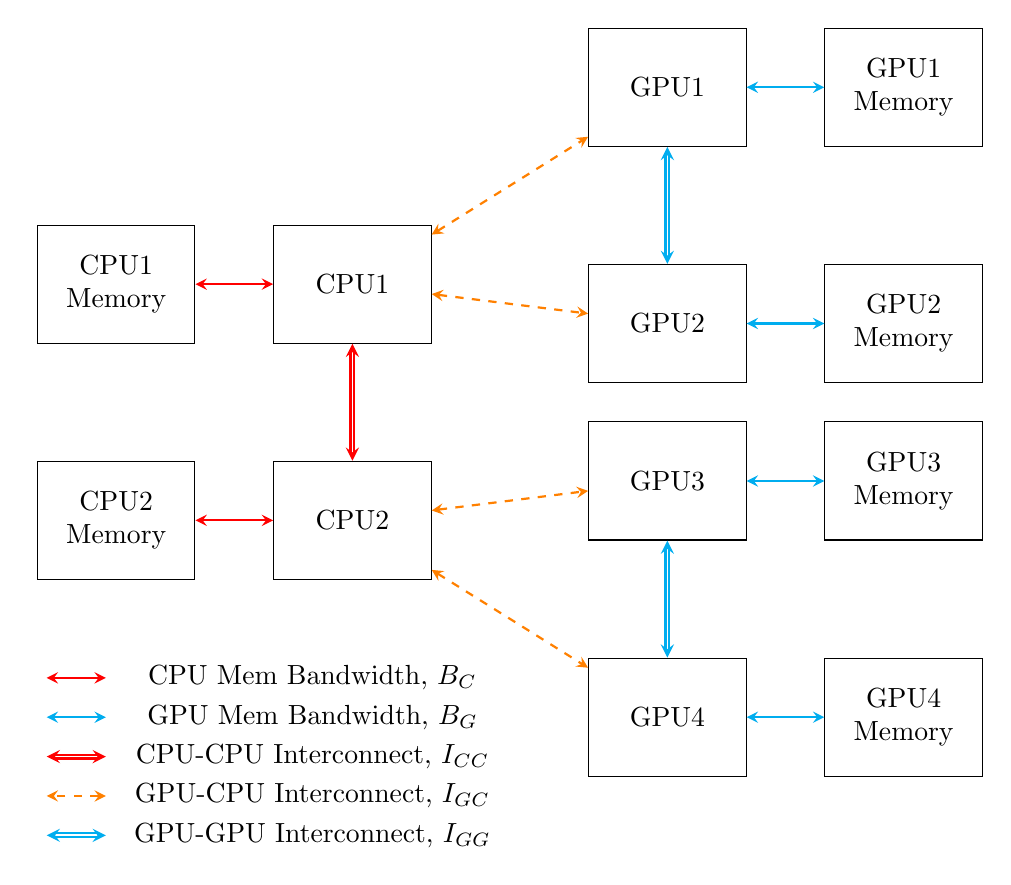
\begin{tikzpicture}
			
			\node[rectangle,
			draw = black,
			text = black,
			anchor = west,
			fill = white,
			align=center,
			minimum width = 2cm, 
			minimum height = 1.5cm] (cpu1) at (0cm,1.5cm) {CPU1};
			
			\node[rectangle,
			draw = black,
			text = black,
			anchor = west,
			fill = white,
			align=center,
			minimum width = 2cm, 
			minimum height = 1.5cm] (cpu2) at (0cm,-1.5cm) {CPU2};
			
			\node[rectangle,
			draw = black,
			text = black,
			anchor = west,
			fill = white,
			align=center,
			minimum width = 2cm, 
			minimum height = 1.5cm] (cpum1) at (-3cm,1.5cm) {CPU1 \\ Memory};
			
			\node[rectangle,
			draw = black,
			text = black,
			anchor = west,
			fill = white,
			align=center,
			minimum width = 2cm, 
			minimum height = 1.5cm] (cpum2) at (-3cm,-1.5cm) {CPU2 \\ Memory};
			
			
			\node[rectangle,
			draw = black,
			text = black,
			anchor = west,
			fill = white,
			align=center,
			minimum width = 2cm, 
			minimum height = 1.5cm] (gpu1) at (4cm,4cm) {GPU1};
			
			\node[rectangle,
			draw = black,
			text = black,
			anchor = west,
			fill = white,
			align=center,
			minimum width = 2cm, 
			minimum height = 1.5cm] (gpu2) at (4cm,1cm) {GPU2};
			
			\node[rectangle,
			draw = black,
			text = black,
			anchor = west,
			fill = white,
			align=center,
			minimum width = 2cm, 
			minimum height = 1.5cm] (gpu3) at (4cm,-1cm) {GPU3};
			
			\node[rectangle,
			draw = black,
			text = black,
			anchor = west,
			fill = white,
			align=center,
			minimum width = 2cm, 
			minimum height = 1.5cm] (gpu4) at (4cm,-4cm) {GPU4};
			
			\node[rectangle,
			draw = black,
			text = black,
			anchor = west,
			fill = white,
			align=center,
			minimum width = 2cm, 
			minimum height = 1.5cm] (gpum1) at (7cm,4cm) {GPU1 \\ Memory};
			
			\node[rectangle,
			draw = black,
			text = black,
			anchor = west,
			fill = white,
			align=center,
			minimum width = 2cm, 
			minimum height = 1.5cm] (gpum2) at (7cm,1cm) {GPU2 \\ Memory};
			
			\node[rectangle,
			draw = black,
			text = black,
			anchor = west,
			fill = white,
			align=center,
			minimum width = 2cm, 
			minimum height = 1.5cm] (gpum3) at (7cm,-1cm) {GPU3 \\ Memory};
			
			\node[rectangle,
			draw = black,
			text = black,
			anchor = west,
			fill = white,
			align=center,
			minimum width = 2cm, 
			minimum height = 1.5cm] (gpum4) at (7cm,-4cm) {GPU4 \\ Memory};
			
			
			\draw[red,  thick, stealth-stealth] (cpum1) to (cpu1);
			\draw[red,  thick, stealth-stealth] (cpum2) to (cpu2);
			\draw[red, double,  thick, stealth-stealth] (cpu1) to (cpu2);
			
			
			\draw[orange, dashed,  thick, stealth-stealth] (cpu1) to (gpu1);
			\draw[orange, dashed,  thick, stealth-stealth] (cpu1) to (gpu2);
			\draw[orange, dashed,  thick, stealth-stealth] (cpu2) to (gpu3);
			\draw[orange, dashed,  thick, stealth-stealth] (cpu2) to (gpu4);
			
			\draw[cyan,  thick, stealth-stealth] (gpum1) to (gpu1);
			\draw[cyan,  thick, stealth-stealth] (gpum2) to (gpu2);
			\draw[cyan,  thick, stealth-stealth] (gpum3) to (gpu3);
			\draw[cyan,  thick, stealth-stealth] (gpum4) to (gpu4);
			
			\draw[cyan, double,  thick, stealth-stealth] (gpu1) to (gpu2);
			\draw[cyan, double,  thick, stealth-stealth] (gpu3) to (gpu4);
			
			
			\node(al) at (-2cm, -3.5cm) {};
			\node (ar) at (-3cm, -3.5cm) {};
			\node[align=left] () at (0.5cm, -3.5cm) {CPU Mem Bandwidth, $B_{C}$};
			\draw[red,  thick, stealth-stealth] (al) to (ar);
			
			\node(al) at (-2cm, -4cm) {};
			\node (ar) at (-3cm, -4cm) {};
			\node[align=left] () at (0.5cm, -4cm) {GPU Mem Bandwidth, $B_{G}$};
			\draw[cyan,  thick, stealth-stealth] (al) to (ar);
			
			\node (bl) at (-2cm, -4.5cm) {};
			\node (br) at (-3cm, -4.5cm) {};
			\node[align=left] () at (0.5cm, -4.5cm) { CPU-CPU Interconnect, $I_{CC}$};
			\draw[red, double,  thick, stealth-stealth] (bl) to (br);
			
			\node (cl) at (-2cm, -5cm) {};
			\node (cr) at (-3cm, -5cm) {};
			\node[align=left] () at (0.5cm, -5cm) { GPU-CPU Interconnect, $I_{GC}$};
			\draw[orange, dashed,  thick, stealth-stealth] (cl) to (cr);
			
			\node (dl) at (-2cm, -5.5cm) {};
			\node (dr) at (-3cm, -5.5cm) {};
			\node[align=left] () at (0.5cm, -5.5cm) { GPU-GPU Interconnect, $I_{GG}$};
			\draw[cyan, double,  thick, stealth-stealth] (dl) to (dr);
			
			
		\end{tikzpicture}
	\end{center}
\caption{Illustration of the universal computing model}
\end{figure}

\subsection{Supercomputers}

For Piz Daint, Summit and Eiger all relevant hardware metrics were collected and compiled to table \ref{fig:datapoints}. Piz Daint and Eiger were chosen, because the systems can be used to test the code. Furthermore Summit is included as it is, at the time of writing this thesis, one of the most capable supercomputers in the world.

\small
\begin{table}[H]
	\begin{center}
		\resizebox{\textwidth}{!}{%
		\begin{tabular}{|@{} c | c | c | c | }
			Constant & Piz Daint \cite{piz_daint} & Summit\cite{summit} & Alps (Eiger) \\ 
			\hline
			\# Nodes & 5704 & 4608 & 1024\\
			\# CPUs & 1 & 2 & 2\\
			CPU Model & Intel E5-2690 v3 \cite{E5-2690} & IBM POWER9 & AMD EPYC 7742\cite{AMDEPYC} \\
			CPU Mem. & 64 GB & 256 GB & ?? \\   
			$B_C$  & 68 GB/s & 170 GB/s & 204.8 GB/s x 2	\\
			$I_{CC}$ & - & 64 GB/s & ?? \\
			Base $GHZ_C$ & 2.9 GHZ & 4 GHZ & 2.25 GHZ\\
			Max $GHZ_C$ & 3.8 GHZ & 4 GHZ & 3.4 GHZ\\
			\# Cores & 12 & 22 & 64 \\
			Architexture & Haswell & POWER9 & AMD Infinity Architecture \\
			SIMD & AVX2 & VSX & AVX2 \\ 
			\# GPUs & 1 & 6 & 0 \\
			GPU Model & NVIDIA P100 \cite{TESLAP100} &NVIDIA V100s \cite{NVIDIA} & - \\
			GPU Mem. Cap. & 16 GB & 16 GB $\times$ 6 & -\\
			$B_G$ & 732 GB/s & 900 GB/s $\times$ 6 & -\\
			$I_{GC}$ & 32 GB/s & 50 GB/s $\times$ 6 & -\\
			$I_{GG}$ & - & 50 GB/s & -\\
			GPU Tflops & 9,3 & 16.5 & -\\
			\# CUDA Cores & 3584 & 5120 & -\\
		\end{tabular}}	
	\end{center}
	\caption{Datapoints of Supercomputers}
	\label{fig:datapoints}
\end{table}



\subsection{Roofline Performance Model} \label{sec:roof}

In a first step it is determined weather the computations are bound by memory bandwidth or the actual performance of the computing unit. The most costly computation is line 6 of the cut method (figure \ref{proc:cut}) with a runtime of $O(32 \times N)$. Oftentimes when an algorithm iterates over a large dataset performing only very little calculations on its individual elements, the limiting factor is the memory. To support this claim, a roofline models for all three systems is established. A roofline model compares arithmetic intensity in flops per byte against the actual performance of the computing chip in flops and can provide insights weather an application is memory or performance bound. 

\subsubsection{Estimating Flops}

For modern hardware, its fairly uncommon to release flops (floating point operations per second) values. Steadily evolving SIMD instruction sets result in varying performance for different implementation details, which in turn are compiled into different assembly instructions. Depending on the algorithm, implementation details and compilation flags the c++ compiler tries to compile ideal assembly instruction sets. SIMD instructions can only be used when there is a contiguous memory access, thus in some cases a poor memory layout choice may lead to a much lower flops. 

For most modern CPU chip architectures AVX is the fastest SIMD instruction set available. The common AVX2 enables the processing of 8 floating point operations per instruction with a cpi\footnote{cycles per instruction} of 0.5. The $cpi$ varies depending on the chip architecture, however all relevant CPU's from figure \ref{fig:datapoints} support a CPI of 0.5 along with AVX2. A lower $cpi$ results in a higher efficiency, as several instructions can be completed in a single cycle. 

Equation \ref{eq:avx} defines a function to estimate the number of gigaflops for a given hardware. $hz$ is the number of cycles which can be completed within a single second by a processing unit, meanwhile $nf$ is the number of floats which can be processed simultaneously in a single instruction using SIMD. Finally $np$ represents the number of processors, where a perfect parallelization is assumed, meaning 100\% of the code can be parallelized.

\small
\begin{table}[H]
	\begin{center}
			\begin{tabular}{@{} c | c | c }
				Variable & Meaning & Unit\\ 
				\hline
				s & second \\
				cl & processor cycle \\
				f & floating point operation \\
				i & instruction \\
				(g)hz & ($10^{12}$) processor cycles per second & ($10^{12}$) cl / s\\
				nf & floating point operations per instruction & f / i\\
				cpi & cycles per instruction & cl / i \\
				(g)flops &  ($10^{12}$) floating point operations per second & ($10^{12}$) f / s\\
				np & number of processors \\
			
		\end{tabular}
	\end{center}
	\caption{Variables to estimate gflops}
	\label{fig:gflops}
\end{table}

\begin{center}
	\begin{equation}\label{eq:avx}
		gflops = ghz * nf * cpi^{-1} * np
	\end{equation}
\end{center}

Since peak flops benchmarks are available for \textit{NVIDIA} P100 and V100s no estimations need to be made on the GPU side.

\subsubsection{Estimating Arithmetic Intensity}

Arithmetic intensity is measured in FLOPS per byte or the number of floating point operations which are computed per byte loaded from memory. The count left part from the cut algorithm (line 6) in figure \ref{proc:cut} can be translated to the following isolated c++ code:

\begin{lstlisting}[language=c++, caption=Counting the particles left of a cut plane, label=Minimal Count Left C++]
	for(auto p= startPtr; p<endPtr; ++p) nLeft += *p < cut;
\end{lstlisting}

Where $p$ is a C-style array which stores the particles position and $nLeft$ stores the number of particles which are smaller than $cut$. The operations per loaded float can be listed as follows:

\begin{enumerate}
	\item Compare particle to cut
	\item Add result to $nLeft$
	\item Increment pointer $p$
	\item Compare pointer $p$ with $endPtr$
\end{enumerate}

Which results in a total of 4 operations. Since a single float is stored using 4 bytes, this computes to 1.0 operations per byte or an arithmetic intensity of four. 

Estimating the arithmetic intensity for the GPU is a lot more complicated as it can vary a lot depending on the specific implementation details. But for now the same arithmetic intensity is assumed for both CPU and GPU. 

Note that SIMD instructions do not influence the arithmetic intensity, as the number of floating point operations per byte remains the same. It just means that a set of operations is executed concurrently. What is however influenced by AVX, is the maximum number of GFLOPS which can be processed by the hardware. If AVX was ignored, the algorithm would clearly not be bound by memory, but by the much lower performance of the processing unit. For this reason it is important to consider SIMD instructions.

\subsubsection{The Plots}

The maximally achievable gflops for Piz Daint are computed as follows: The datapoints from figure \ref{fig:datapoints} are plugged into the formula \ref{eq:avx} for $np = 2, 4$ and $8$.

\begin{center}
	\begin{equation}
		3.8 \times 10^{12} cl/s \times 8 f/i \times \frac{1}{0.5} i/cl \times 2  = 121.6 gflops
	\end{equation}
	\label{eq:daintp1}
\end{center}

\begin{center}
	\begin{equation}
		3.8 \times 10^{12} cl/s \times 8 f/i \times \frac{1}{0.5} i/cl \times 4 = 243.2 gflops
	\end{equation}
	\label{eq:daintp2}
\end{center}

\begin{center}
	\begin{equation}
	3.8 \times 10^{12} cl/s \times 8 f/i \times \frac{1}{0.5} i/cl \times 8 = 486.4 gflops
	\end{equation}
	\label{eq:daintp3}
\end{center}

The results are depicted as horizontal lines in figure \ref{fig:roofdaint}. The memory bandwidth is plotted as a line with an equivalent slope. Finally a dotted line represents the arithmetic intensity of the Count Left procedure. 
To interpret the roofline mode, one has to follow the dotted line starting from the bottom. Weather it intersect with line representing the maximal performance or the memory bandwidth first, gives an indication weather the program is performance or memory bound. 

\begin{figure}[H]
	\begin{center}
		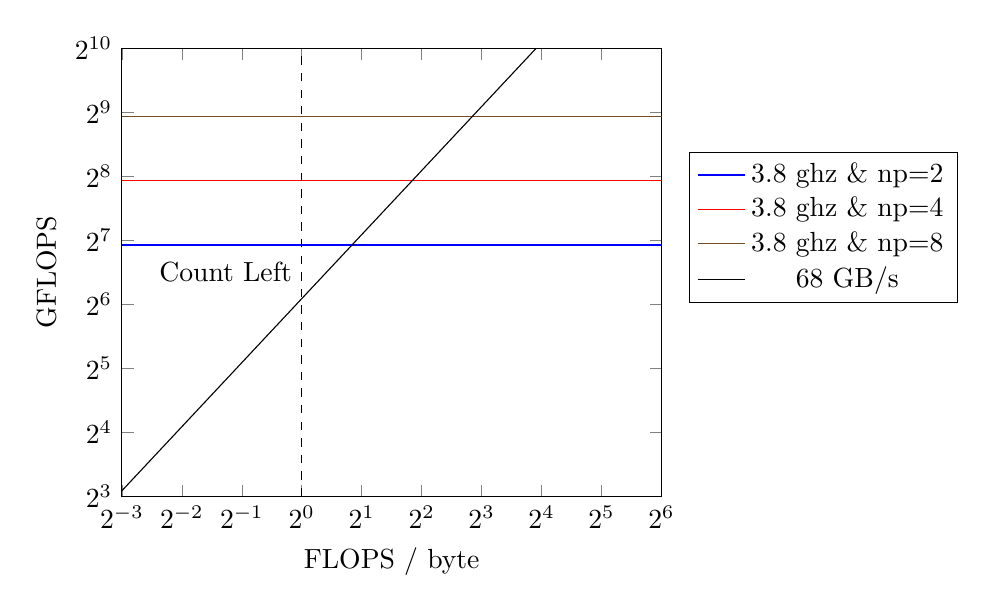
\begin{tikzpicture}
				\begin{axis}[
					xmode=log,
					ymode=log,
					log basis x={2},
					log basis y={2},
					xlabel={FLOPS / byte},
					ylabel={GFLOPS},
					%x filter/.code=\pgfmathparse{#1 + 6.90775527898214},
					xmin = 0.125, xmax = 64, ymin= 8, ymax=1024,
					legend style={at={(1.05,0.6)},anchor=west}]
			
					\addplot+[name path = A, domain = 0.125:64, mark=none] {
						3.8 * 8 * 2 * 2
					};	
					
					\addlegendentryexpanded{3.8 ghz \& np=2};
					
					\addplot+[name path = A, domain = 0.125:64, mark=none] {
						3.8 * 8 * 2 * 4
					};	
					
					\addlegendentryexpanded{3.8 ghz \& np=4};
					
					\addplot+[name path = A, domain = 0.125:64, mark=none] {
						3.8 * 8 * 2 * 8
					};	
					
					\addlegendentryexpanded{3.8 ghz \& np=8};
					
					\addplot+[name path = A, domain = 0.125:64, mark=none] {
						68 * \x
					};	
					
					\addlegendentryexpanded{68 GB/s};
					
		
					\draw[dashed] (axis cs:1,8) -- node[left]{Count Left} (axis cs:1,1024);
					
				\end{axis}
			\end{tikzpicture}
	\caption{Roofline Model for Piz Daint CPU}
	\label{fig:roofdaint}
	\end{center}
\end{figure}


\begin{figure}[H]
	\begin{center}
		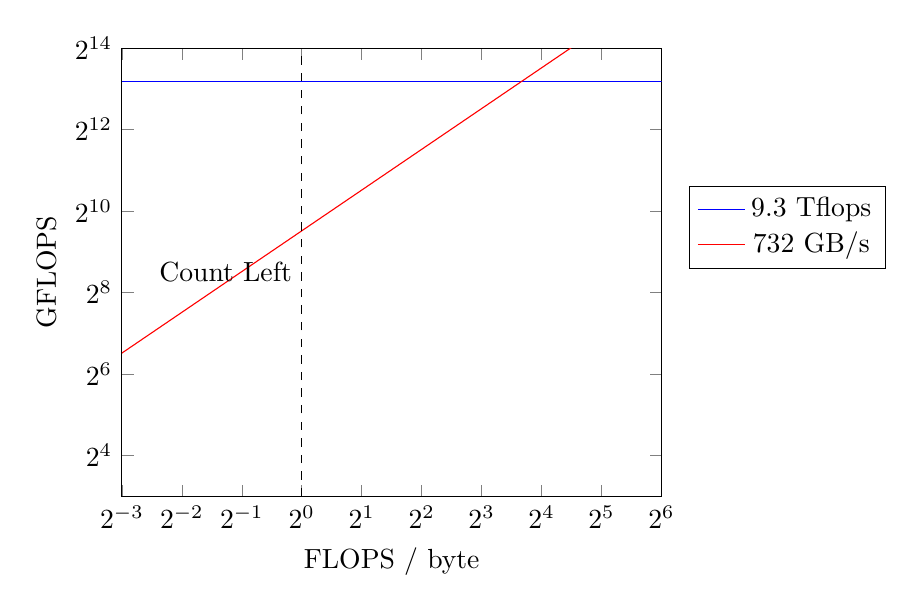
\begin{tikzpicture}
			\begin{axis}[
				xmode=log,
				ymode=log,
				log basis x={2},
				log basis y={2},
				xlabel={FLOPS / byte},
				ylabel={GFLOPS},
				%x filter/.code=\pgfmathparse{#1 + 6.90775527898214},
				xmin = 0.125, xmax = 64, ymin= 8, ymax=16384,
				legend style={at={(1.05,0.6)},anchor=west}]
				
				\addplot+[name path = A, domain = 0.125:64, mark=none] {
					9300
				};	
				
				\addlegendentryexpanded{9.3 Tflops};
				
				\addplot+[name path = A, domain = 0.125:64, mark=none] {
					732 * \x
				};	
				
				\addlegendentryexpanded{732 GB/s};
				
				
				\draw[dashed] (axis cs:1,8) -- node[left]{Count Left} (axis cs:1,16384);
				
			\end{axis}
		\end{tikzpicture}
		\caption{Roofline Model for Piz Daint GPU}
		\label{fig:roofdaintGPU}
	\end{center}
\end{figure}

As it can be seen in figure \ref{fig:roofdaint} and \ref{fig:roofdaintGPU} both the GPU and CPU version running on Piz Daint are memory bound, but due to its much higher memory bandwidth limit, a GPU version should be favored. 

\begin{figure}[H]
	\begin{center}
		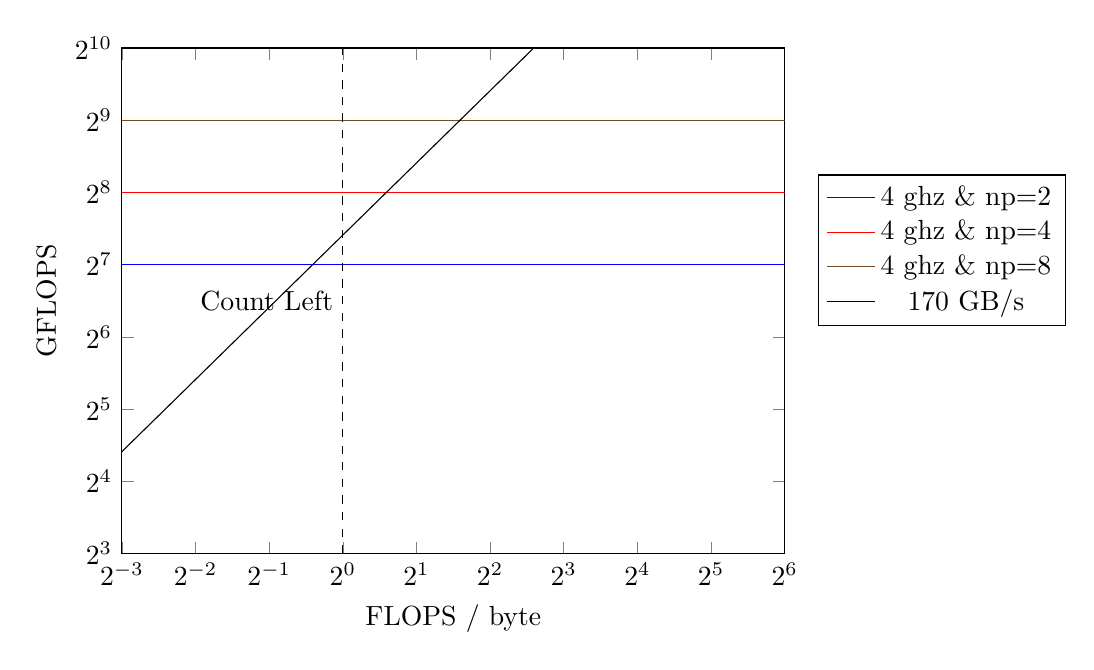
\begin{tikzpicture}
			\begin{axis}[
				xmode=log,
				ymode=log,
				log basis x={2},
				log basis y={2},
				height=8cm,width=10cm, 
				xlabel={FLOPS / byte},
				ylabel={GFLOPS},
				%x filter/.code=\pgfmathparse{#1 + 6.90775527898214},
				xmin = 0.125, xmax = 64, ymin= 8, ymax=1024,
				legend style={at={(1.05,0.6)},anchor=west}]
				
				
				\addplot+[name path = A, domain = 0.125:64, mark=none] {
					4 * 8 * 2 * 2
				};	
				
				\addlegendentryexpanded{4 ghz \& np=2};
				
				\addplot+[name path = A, domain = 0.125:64, mark=none] {
					4 * 8 * 2 * 4
				};	
				
				
				\addlegendentryexpanded{4 ghz \& np=4};
				
				\addplot+[name path = A, domain = 0.125:64, mark=none] {
					4 * 8 * 2 * 8
				};	
				
				
				\addlegendentryexpanded{4 ghz \& np=8};
				
				\addplot+[name path = A, domain = 0.125:64, mark=none] {
					170 * \x
				};	
				
				\addlegendentryexpanded{170 GB/s};
				
				
				\draw[dashed] (axis cs:1,8) -- node[left]{Count Left} (axis cs:1,1024);
			
				
			\end{axis}
		\end{tikzpicture}
	\end{center}
	\caption{Roofline Model for Summit}
	\label{fig:roofsummit}
\end{figure}


\begin{figure}[H]
	\begin{center}
		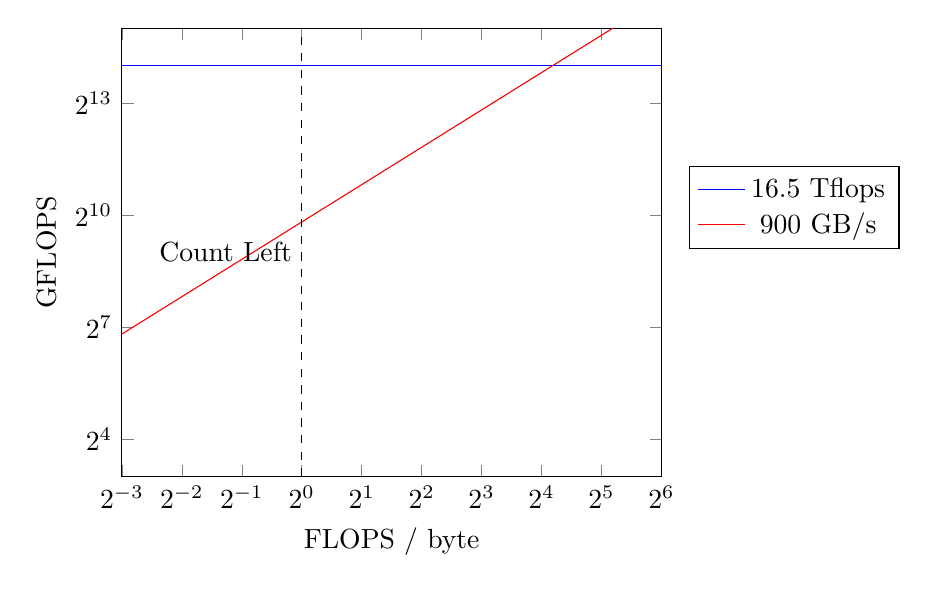
\begin{tikzpicture}
			\begin{axis}[
				xmode=log,
				ymode=log,
				log basis x={2},
				log basis y={2},
				xlabel={FLOPS / byte},
				ylabel={GFLOPS},
				%x filter/.code=\pgfmathparse{#1 + 6.90775527898214},
				xmin = 0.125, xmax = 64, ymin= 8, ymax=32768,
				legend style={at={(1.05,0.6)},anchor=west}]
				
				\addplot+[name path = A, domain = 0.125:64, mark=none] {
					16500
				};	
				
				\addlegendentryexpanded{16.5 Tflops};
				
				\addplot+[name path = A, domain = 0.125:64, mark=none] {
					900 * \x
				};	
				
				\addlegendentryexpanded{900 GB/s};
				
				
				\draw[dashed] (axis cs:1,8) -- node[left]{Count Left} (axis cs:1,32768);
				
			\end{axis}
		\end{tikzpicture}
		\caption{Roofline Model for Summit GPU}
		\label{fig:roofsummitGPU}
	\end{center}
\end{figure}

As visible in figure \ref{fig:roofsummit} and \ref{fig:roofsummitGPU} the same applies to Summit. Its notable how the memory bandwidth only becomes the limiting factor when assuming a parallelization with 4 processors.

\begin{figure}
	[H]
	\begin{center}
		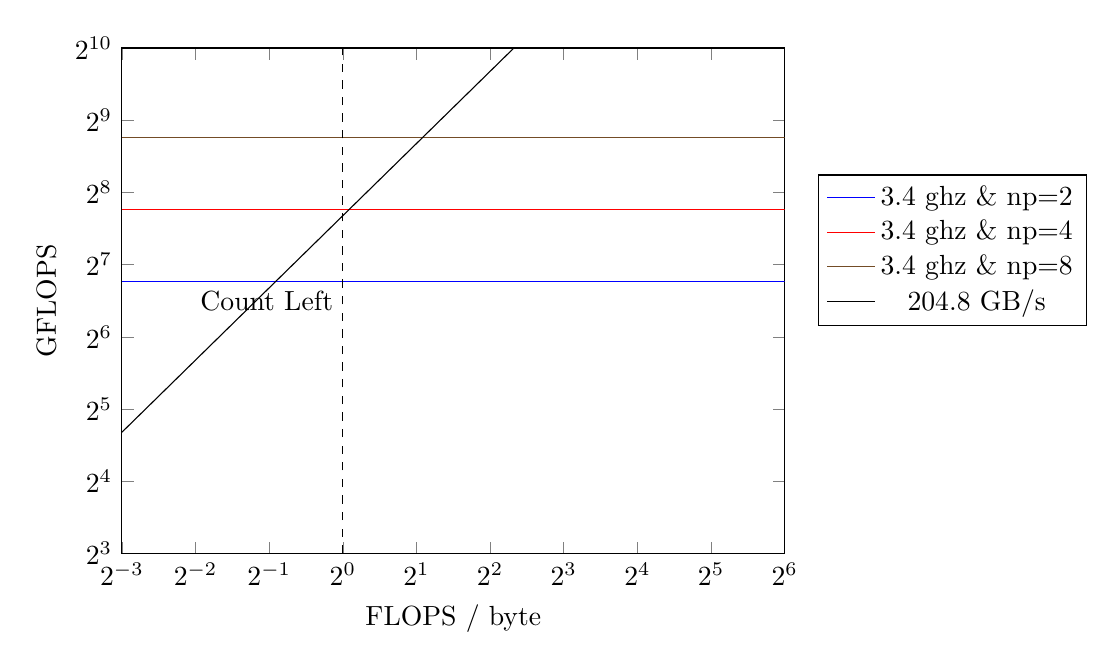
\begin{tikzpicture}
			\begin{axis}[
				xmode=log,
				ymode=log,
				log basis x={2},
				log basis y={2},
				height=8cm,width=10cm, 
				xlabel={FLOPS / byte},
				ylabel={GFLOPS},
				%x filter/.code=\pgfmathparse{#1 + 6.90775527898214},
				xmin = 0.125, xmax = 64, ymin= 8, ymax=1024,
				legend style={at={(1.05,0.6)},anchor=west}]
				
				
				\addplot+[name path = A, domain = 0.125:64, mark=none] {
					3.4 * 8 * 2 * 2
				};	
				
				\addlegendentryexpanded{3.4 ghz \& np=2};
				
				\addplot+[name path = A, domain = 0.125:64, mark=none] {
					3.4 * 8 * 2 * 4
				};	
				
				\addlegendentryexpanded{3.4 ghz \& np=4};
				
				\addplot+[name path = A, domain = 0.125:64, mark=none] {
					3.4 * 8 * 2 * 8
				};	
				
				\addlegendentryexpanded{3.4 ghz \& np=8};
				
				\addplot+[name path = A, domain = 0.125:64, mark=none] {
					204.8 * \x
				};	
				
				\addlegendentryexpanded{204.8 GB/s};
				
				\draw[dashed] (axis cs:1,8) -- node[left]{Count Left} (axis cs:1,1024);
				
				
			\end{axis}
		\end{tikzpicture}
	\end{center}
	\caption{Roofline Model for Alps}
	\label{fig:roofalps}
\end{figure}

Finally alps, which has the highest memory bandwidth compared to its flops, also becomes limited by the memory bandwidth after using more than four processors.

\subsubsection{Empirical Verification}

A minimal C++ code is considered to verify the theoretical model. The -S flag along with the g++ compiler is used to generate assembly code from the c++ source code. For testing purposes all entries in the array are set to random values between 0 and 1, and $cut$ is set to 0.5.

In a first test, only $O3$ is enabled. The generated assembly code is depicted in listing \ref{assembler}.

\begin{lstlisting}[language=c++, caption=Reduction Assembler Code without AVX, label=assembler]
.L18:
	movups	(%rax), %xmm0
	addq	$16, %rax
	cmpltps	%xmm2, %xmm0
	psubd	%xmm0, %xmm1
	cmpq	%rdx, %rax
	jne	.L18

\end{lstlisting}

$psubd$ is a packaged instruction, meaning it already uses some form of SIMD instructions. The command is used in the MME and later the SSE2 instruction set. Since the $xmm$ registers are used, it follows that it is an AVX instruction.

If the compile flag $-march=native$ is added, the instructions as depicted in listing \ref{assembler-avx} are the result of the compilation.

\begin{lstlisting}[language=c++, caption=Reduction Assembler Code with AVX2, label=assembler-avx]
.L19:
	vmovups	(%rax), %ymm3
	addq	$32, %rax
	vcmpltps	%ymm2, %ymm3, %ymm0
	vpsubd	%ymm0, %ymm1, %ymm1
	cmpq	%rdx, %rax
	jne	.L19	

\end{lstlisting}

$vmovups$, $vcomplpts$ and $vpsubd$ are AVX2 commands since they are using the $ymm$ registers.

The following results were obtained on $2^{27}$ particles with a thread count of 16 on Piz Daint. The reduction takes 2.3 milliseconds, resulting in a throughput of $2^{27} / 10^{9} * 10^3 / 2.3 = 58 gflops$. This is close to the memory bandwidth (68 GB/s) and far below the performance maximum of the CPU, which even for ($np = 1$) is $3.8 * 8 * 2 * 1 * 16 = 972.8 gflops$. Thus the algorithm is assumed to be memory bound for the CPU and most probably memory bound for the GPU. 


\subsection{Runtime Estimates}

A runtime estimation for the CPU version and two different GPU implementations is constructed. In the first GPU implementation \textit{GPU Counting}, an array of particles is sent to the GPU, where counting is then performed. In a more advanced variant \textit{GPU Counting and Partitioning} the particles are sent from the CPU to GPU only once and the partitioning is performed on the GPU as well.  

A precision $p$ of 32 is assumed, which is a sensible assumption for astrophysical simulations. The total storage required for all particle positions is $32 \times 3 \times N bits = 4 \times 3 \times N Bytes = 12 \times N Bytes$. Furthermore $d = 1024$ and $N=10^9$ are assumed.
 
\subsubsection{CPU Version}

Each time the leaf cells of the SPTDS are split into two child cells and appended to the tree, the tree ends up with twice the number of cells. As the goal is to construct a tree with $d$ leaf cells, the cut algorithm needs to be performed $\lceil log_2(d) \rceil$ times over all leaf cells. 

\small
\begin{table}[H]
	\begin{center}
		\begin{tabular}{@{} c | c | c }
			Variable & Meaning & Unit\\ 
			\hline
			$d$ & number of leafs cells in the final SPTDS \\
			$p$ & precision of each coordinate (number of bits) \\
			$s$ & data size of all particle coordinates \\
			$B_C$ & memory bandwidth between the CPU and its memory & GB/s \\
			$B_G$ & memory bandwidth between the GPU and its memory & GB/s \\
			$B_G$ &	memory bandwidth between the CPU and the GPU & GB/s \\
	
			
		\end{tabular}
	\end{center}
	\caption{Variables used for runtime estimates}
	\label{tab:runtime}
\end{table}

Consequently the runtime estimate sums over all $\lceil log_2(d) \rceil$ iterations, where in each iteration a cut has to be found for $i$ cells. The cut for a single cell is found in $p$ iterations, where the number of particles to be iterated over for a single cell is divided by two in each iteration. 



\begin{center}
	\begin{equation}
		\sum_{i=1}^{\lceil \log_2{d} \rceil} i \times p \times  \frac{ \frac{s}{i}}{B_C} 
		\label{eq:cpu1}
	\end{equation}
\end{center}

$i$ cancels out from the equation and the equation becomes:

\begin{center}
	\begin{equation}
		\sum_{i=1}^{\lceil \log_2{d} \rceil} p \times \frac{s}{B_C} 
		\label{eq:cpu2}
	\end{equation}
\end{center}

Which can be simplified to:

\begin{center}
	\begin{equation}
		\lceil \log_2(d) \rceil  \times \left ( p \times \frac{ s }{B_{C}} \right )
		\label{eq:cpu}
	\end{equation}
\end{center}

\subsubsection{GPU Counting}


The Equation \ref{eq:gpu} for the GPU is similar, the only difference being that  GPU memory bandwidth $B_{GPU}$ is used instead of the CPU bandwidth. Furthermore the additional overhead of sending the data from the CPU to the GPU has to be reflected. This adds the terms size divided by CPU to GPU memory bandwidth denoted as $I_{GC}$.

\begin{center}
	\begin{equation}
			\lceil log(d) \rceil \times \left ( p \times \frac{s}{B_{G}} +\frac{s}{I_{GC}} \right ) 
		\label{eq:gpu}
	\end{equation}
\end{center}


\subsubsection{GPU Counting and Partitioning}\label{gpu-tree-building}

Another variant is to perform the partitioning on the GPU, meaning there is no need to send data from the CPU to the GPU each time a cut needs to be found. This allows for a reduction of the costly overheads introduced by the rather slow bandwidth $I_{GC}$. The overhead can be moved out of the bracket as the transfer needs to happen only once before. 

\begin{center}
	\begin{equation}
		\lceil log(d) \rceil \times \left ( p \times \frac{s}{B_{G}} \right ) + \frac{s}{I_{GC}} = t
		\label{eq:gputree}
	\end{equation}
\end{center}

\newcommand\s{12}

\newcommand\p{32}

%\newcommand\d{1024}

\normalfont
\subsubsection{Plugin Values} 

Lets plugin the values from figure \ref{fig:datapoints} into the corresponding formulas \ref{eq:cpu}, \ref{eq:gpu} and \ref{eq:gputree} for Piz Daint.
The following values and consequently speed up can be computed for CPU only version:

\pgfmathsetmacro\cpuPiz{ln(1024) / ln(2) * (\p * \s / 68)}

\begin{center}
	\begin{equation}
		\lceil log(1024) \rceil \times \left ( \p \times \frac{ \s GB }{68 GB/s} \right )  = \cpuPiz s
	\end{equation}
\end{center}


Whereas a GPU accelerated Count Left results in the following runtime:
\pgfmathsetmacro\gpuPizN{ ln(1024) / ln(2) * (\p * \s / 732 + \s / 32)}
\begin{center}
	\begin{equation}
		\lceil log(1024) \rceil \times \left ( 32 \times \frac{12 GB}{732 GB/s} + \frac{12 GB}{32 GB/s} \right )=  \gpuPizN s
	\end{equation}
\end{center}

This yields in a speed-up of the GPU over the CPU only version:
\pgfmathsetmacro\speedup{\cpuPiz / \gpuPizN}
\begin{center}
	\begin{equation}
		\frac{\cpuPiz}{\gpuPizN} = \speedup \times
	\end{equation}
\end{center}


When considering the GPU Counting and Partitioning the results are:
\pgfmathsetmacro\gpuPizT{ ln(1024)/ln(2) * (\p * \s / 732)  + \s / 32}
\begin{center}
	\begin{equation}
		\lceil log(1024) \rceil \times \left ( \p \times \frac{\s GB}{732 GB/s} \right ) + \times \frac{\s GB}{32 GB/s} = \gpuPizT s
	\end{equation}
\end{center}

This yields in a speed-up over the CPU obly version of:
\pgfmathsetmacro\speedup{\cpuPiz / \gpuPizT}
\begin{center}
	\begin{equation}
		\frac{\cpuPiz}{\gpuPizT} = \speedup \times
	\end{equation}
\end{center}

\vspace{5mm}

\pgfmathsetmacro\cpuSummit{ln(1024) / ln(2) * (\p * \s / (170 * 2)}
\pgfmathsetmacro\gpuSummitN{ln(1024) / ln(2) * (
	(\p * \s / (900 * 6) + 
	\s / (50 * 6)
	)}
\pgfmathsetmacro\gpuSummitT{ln(1024) / ln(2) * 
	(\p * \s / (900 * 6))
	+  \s / (50 * 6)}
\pgfmathsetmacro\cpuEiger{ln(1024) / ln(2) * (\p * \s / (204.8 * 2)}


\subsection{Conclusion}

 
The computations for Eiger and Summit can be performed analogously to the ones from Piz Daint. Eiger is non hybrid, thus only estimates for a CPU version are computed. All the results are plotted in \ref{fig:exectimes}. As expected the GPU Counting outperforms the CPU version on both hybrid\footnote{Each node has a CPU and a GPU} super computers. Furthermore GPU Counting and Partitioning yields more performance improvements, but the speed up is less drastic. As the model may differ from reality depending on the implementation and compilation details, these results cannot be taken for granted but offer a good baseline of what is possible. 

\begin{figure}[H]
	\begin{center}
		\begin{tikzpicture}
			
			\begin{axis} [ybar,height=10cm,width=13cm, 
				bar width=0.8cm,
				enlarge x limits=0.2,
				ymin = 0,
				ymax = 60,
				symbolic x coords={Piz, Summit, Eiger},
				legend columns=1,
				legend entries={CPU, Hybrid Naive, Hybrid Tree},
				ylabel={Runtime (s) },
				x tick label style={rotate=45,anchor=east}, 
				xtick=data]
				\addplot coordinates {
					(Piz,\cpuPiz ) 
					(Summit,\cpuSummit) 
					(Eiger,\cpuEiger) 
				};
			
				\addplot coordinates {
					(Piz,\gpuPizN ) 
					(Summit,\gpuSummitN ) 
				};
			
				\addplot coordinates {
					(Piz,\gpuPizT ) 
					(Summit,\gpuSummitT  ) 
				};
			\end{axis}
			
		\end{tikzpicture}
	\end{center}

\caption{Estimated runtimes of different variants}
\label{fig:exectimes}
\end{figure}


\newpage
\section{CPU Implementation}

In this section the stand-alone implementation of the ORB algorithm using CPU acceleration only is described. Building on the CPU version, GPU accelerated alternatives to selected parts of the code are proposed. 

The code is developed somewhat separately from the PKDGrav codebase in order to keep the project smaller and more easy to understand. However the machine dependent layer (MDL) from PKDGrav is used, which provides a system to distribute the workload among processors. This reduces the complexity of the implementation because communication and CPU parallelism are abstracted away from the code. Furthermore it makes integration into PKDGrav simple.
Not every part of the code is described in detail, however any details crucial to performance are outlined. Furthermore, special attention is paid to the CUDA kernels and memory management strategies for two reasons: minor implementation details can have a big impact upon the performance and increased replicability.

For this project C++ 17 along with CUDA 11.3, OpenMPI 4.1.0 and Blitz++ 1.0.2  \cite{blitzcpp} is used. 

\subsection{MDL and PKDGrav}

MDL, the machine dependent layer provides an abstraction layer around the parallel primitives introduced by PKDGrav. The Master layer is responsible to coordinate the flow of the program. It does so by calling the PST (Processor Set Tree), which distributes the tasks and gets processors to work on them. As the name suggests, the PST is organized as a binary tree where intermediate nodes contain a pointer to a consecutive processor as well as a next lower node. Each leaf cell of the graph then correspond to an individual core.

Parallel processes are dispatched by descending the PST until they reach all processors. There computations are performed and the results are combined by passing them back up the PST until they reach the master.
A parallel process can be programmed by implementing the service interface as explained in section \ref{services}.

Each processor has its own local data, which can be accessed by calling $pst->lcl$. 

\subsection{Particles}

The particles array has ownership over all particle objects. It has a (N,3) shape where as each row represents a single particle. To enable coalesced memory access when iterating over a single axis i.e. $x_{:, axis}$, a column major storage order is chosen, meaning that each column is stored in a range of consecutive array addresses. Even though row accesses patterns i.e. $x_{i,:}$ are used as well, they happen less frequently. Most importantly there are cases where where entire sections of a row has to be copied. This is by magnitudes faster with a row major storage.

C-style arrays are used interchangeably with Blitz++ arrays to store all particles. Blitz++ is an open source wrapper class around C-style arrays, which helps with pointer management and can speed up the debugging process by keeping track of the array boundaries. Furthermore, it features array slicing and does its own memory management. In certain cases the actual C-style arrays needs to be accessed, which can be accessed by calling $array.data()$. For example when iterating over the Blitz++ array, non optimal assembly code was observed, not reflecting optimal SIMD instructions available to the hardware. 

The particle data is loaded into the local data storage of each processor, meaning each processor owns a different unique set of particles.

\subsection{Cell}

The cell class is a structure keeping track of the fundamental cell information. In essence it is the analogue to the concept of the $cell$ which has been introduced in section \ref{section:orb}.

Quickly building and accessing elements of the SPTDS generated by ORB requires a suitable data structure. Instead of a tree with pointers, a heap can be used since the necessary conditions for a nearly complete binary tree are met. Elements within a heap can be accessed and added in constant runtime. Depicted in figure \ref{fig:treeheap} is the finished SPTDS of the sample dataset stored as a heap.

The SPTDS and thus the cells are constructed on the master alone. Cells are only distributed when dispatching services on the PST.

\begin{figure}[H]
	\begin{center}
		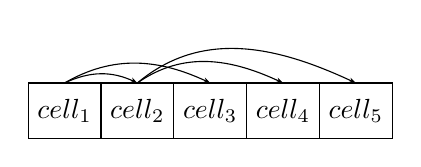
\begin{tikzpicture}[
			%  -{Stealth[length = 2.5pt]},
			start chain = going right,
			node distance = 0pt,
			MyStyle/.style={draw, minimum width=2em, minimum height=2em, 
				outer sep=0pt, on chain},
			]
			\node [MyStyle] (1) {$cell_1$};
			\node [MyStyle] (2) {$cell_2$};
			\node [MyStyle] (3) {$cell_3$};
			\node [MyStyle] (4) {$cell_4$};
			\node [MyStyle] (5) {$cell_5$};
			\begin{scope}[-{Stealth[length = 2.5pt]}]
				\draw (1.north) [out=25, in=155] to (2.north);
				\draw (1.north) [out=30, in=155] to (3.north);
				\draw (2.north) [out=35, in=155] to (4.north);
				\draw (2.north) [out=40, in=155] to (5.north);
			\end{scope}
		\end{tikzpicture}
		\qquad
		\begin{figure}
			\Tree[.cell_1 [.cell_2 [.cell_4 ] [.cell_5 ] ]
			[.cell_3 ]]
		\end{figure}
	\end{center}
	\caption{Tree as heap}
	\label{fig:treeheap}
\end{figure}

An array can be used as an efficient storage medium for the heap, since in this case $d$, the number of leafs cells in the final SPTDS, can be set at compile time and the maximum number of cells in the SPTDS can be derived from that. Meaning the array can be allocated statically.
Because MDL communicates data as arrays between threads, another advantage of the array storage is the absence of any costly data structure conversion. 

Since the STPDS is only a nearly complete binary tree and not a complete binary tree, special attention has to be paid when performing the ORB algorithm in an iterative way. But because $d$ is known, many attributes of the SPTDS can be determined deterministically.

\subsubsection{Heap Conditions}
As with all heap data-structures the following conditions are given:

\begin{itemize}
	\item The root cell has an index 1
	\item The left child of a cell at index $i$ can be accessed at the index $i\times2$. 
	\item The left child of a cell at index $i$ can be accessed at the index $i\times2 + 1$. 
\end{itemize}

\begin{figure}[H]
	\centering
	\begin{forest}
		[$cell_1$
		[$cell_2$ [$cell_4$] [$cell_5$]][$cell_3$]  
		]
	\end{forest}
	\caption{Tree with $d$ = 3}
	\label{fig:extree}
\end{figure}

\vspace{0.5cm}
The following constraints can be derived given the number of leaf cells $d$. 

\begin{itemize}
	\item The depth of the tree can be computed with: $\lceil log_2(d) \rceil$
	\item The number of leaf cells on the second last level is given by $2^{depth} - d$ 
	\item There are exactly $2 \times d - 2^{depth}$ items (which must all be leaf cells) on the last level. 
	\item The total number of cells are $2\times d - 1$.
\end{itemize}

In the example tree depicted in figure \ref{fig:extree} the depth corresponds to: $\lceil log_2(d) \rceil = 2$, the number of leaves on the second last level is  $2^{2} - 3 = 1$ and the number of leaves on the last level are $2 \times 3 - 2^{2} = 2$. Finally the total number of cells is $2\times 3 - 1 = 5$.

\subsubsection{Class}
Among the fields in the cell are the following variables:

\begin{itemize}
	\item $id$ is the unique identification of the cell instance. It corresponds to its index in the heap array plus one. The plus one comes from the different indexing for heap constraints, starting with 1, and the classic array indexing starting with 0. It can be used to compute  indices of both child cells and parent cells using the above shown formulas.
	\item $nLeafCells$ is equivalent to  $d_{cell}$ and depicts the number of leaf cells to be found in all of its successors. Its used when building the tree, to track weather a cell needs to be split or not. 
	\item $lower$ is a 3D point coordinate representing the lower boundary corner of the 3D volume $V_{cell}$ which is encompassed by this cells.
	\item $upper$ represents the upper boundary corner of the volume.	
	\item $cutAxis$ is the axis where the cell is to be cut. 
\end{itemize}

To support and simplify common operations, a further abstraction layer is given with the following functions:


\begin{itemize}
	\item $setCutAxis()$ evaluates the proper $cutAxis$ given the $upper$ and $lower$ variables.
	\item $cut()$ cuts the cell and returns two new cells. 
	\item $getLeftChildId()$ returns the ID of the left child cell, meaning its volume is in the cut axis smaller than the cut plane. 
	\item $getRightChildId()$ is the equivalent for the right child. 
\end{itemize} 

\subsection{Mapping Cells to Particles}

As the SPTDS heap is stored on the master but the particles are distributed among the local storages of the processors, its is crucial to know which particles are encompassed in the volume of which cell. Thus a data structure to keep track of the relation between cells and its particles is introduced.
Thanks to the partitioning algorithm all particles belonging to a single cell can be found in a consecutive section of the particles array. A 2D array is used to keep track of the relation, which again is stored in the local data of the processor. For each cell the corresponding section is stored as a tuple of begin and end indices. Naturally the data structure needs to be updated across all processors whenever a partition is performed.

\subsection{Services}\label{services}

A service implementation consists of a $Service()$ function as well as a $Combine()$ function. Parameters include an $PST$ object which stores information about the process location as well as the local data. Furthermore two void pointers providing storage for the input and output data called $in$ and $out$ along with their respective sizes are passed. The reason void pointers are used, is the variability of the input data structures. C++ does not offer dynamic typing. Data stored inside the void pointers can be converted into their respective classes using casting. 

In the $Combine()$ function two output void pointers $vout$ and $vout2$ and the sizes of the underlying arrays are given as parameters. A combination strategy of the elements can be chosen and implemented, where the results is to be stored in $vout$. For example in a service which returns the sum of all particles, the combine function would simply store the sum of $vout$ and $vout2$ in $vout$.

\subsubsection{Init and Finalize Service}

All data stored in the local memory of a PST, must be allocated when initializing the program. After the program has finished, the memory is freed to avoid any leaks. Allocation and freeing comes with some overhead, thus it makes sense to reuse memory whenever possible. 

The initialize service is also responsible to load the particle data into the local memory of each PST. 

\subsubsection{Count Left Service}

As mentioned, counting the elements smaller than the cut position is computationally intensive. 
The $Service()$ function which performs the actual computations, $in$ points to an array of cells and as the length of the array is known, its possible to simply iterate over all of its elements and cast them to the correct cell data structure as shown in listing \ref{ctl} on line 1-2. In case the $foundCut$ flag of cell was set to true, its known that the ideal cut was already found and the cell can be skipped (line 4-6).
Then the begin and end indices of the particles array corresponding to the range of objects contained within the cells volume are read and respectively a slice of the local particles array (lines 7-11) is made. Start and end pointers are computed and the cut position to be tested is fetched (lines 13 -17). Finally the number of particles smaller than the cut are counted and written back to the output array (lines 18-23). As the results for each cell needs to be stored individually, its written to the output with an offset equivalent to the $cellPtrOffset$. This offset however does not corresponds to the $cell.id$, its rather a sequential indexing over all leaf cells of the same depth in the SPTDS. 


\begin{lstlisting}[language=c++, caption=Part of the Count Left Service() method, label=ctl]
for (int cellPtrOffset=0; cellPtrOffset<nCells; ++cellPtrOffset){
	auto cell = static_cast<Cell>(*(in + cellPtrOffset));
	
	if (cell.foundCut) {
		continue;
	}
	int beginInd = pst->lcl->cellToRangeMap(cell.id, 0);
	int endInd =  pst->lcl->cellToRangeMap(cell.id, 1);
	
	blitz::Array<float,1> particles =
	pst->lcl->particlesAxis(blitz::Range(beginInd, endInd));
	
	float * startPtr = particles.data();
	float * endPtr = startPtr + (endInd - beginInd);
	
	int nLeft = 0;
	float cut = cell.getCut();
	for(auto p= startPtr; p<endPtr; ++p)
	{
		nLeft += *p < cut;
	}
	
	out[cellPtrOffset] = nLeft;
}
\end{lstlisting}

Combining the data is straight forward, as in $Combine()$ $vout$ and $vout2$ contain the counts for a given number of particles. The master requires a global count across all the particles contained within all local storages, therefore each element of $vout$ is summed together with $vout2$. 

\begin{lstlisting}[language=c++, caption=Part of the Count Left Combine() method, label=ctlc]
	for(auto i=0; i<nCounts; ++i)
		out[i] += out2[i];
\end{lstlisting}

\subsubsection{Count}

Counting the total number of particles contained within a cell is trivial with the $cellToRangeMap$. The results can be obtained by subtracting the begin index from the end index of each cell. The $Combine()$ is equal to the one shown for the Count Left Service.

\begin{lstlisting}[language=c++, caption=Part of Count Service() method]
	for (int cellPtrOffset=0; cellPtrOffset<nCells; ++cellPtrOffset) {
		auto cell = static_cast<Cell>(*(in + cellPtrOffset));
		out[cellPtrOffset] = 
		lcl->cellToRangeMap(cell.id,1) - 
		lcl->cellToRangeMap(cell.id,0);
	}
\end{lstlisting}

\subsubsection{Partition}

The Partitioning Service is a direct implementation of the hoare partition and can be seen in listing \ref{partition}. Again the service receives a buffer with a given number of cells, which are then iterated over using the outer for loop. Each cell from the buffer is then casted to the proper struct (line 2). Using the id of the cell, the start and end indices of the corresponding particles stored in local storage can be accessed (lines 4-5). Lines 7-37 search for pairs located on the wrong side of the cut and then swap them using a simple $swap()$ helper function. $i$ has to be initialized using $beginInd -1$ as the $i++$ operation happens before a read on the array (line 15). For the same reason $j$ is initialized to $endInd$ and not $endInd -1$. Then the while loop terminates, $i$ points to the first index in the array where the value is greater than the cut, therefore $cellToRangeMap$ can be updated using $i$, as for the left child cell the start remains equal but the end is now $i$ and for the right child cell its vice versa. 
Note that the implementation is not ideal for two reasons:

\begin{enumerate}
	\item The blitz wrapper class should be avoided and instead the memory directly accessed.
	\item In this particular case the column major storage order is not ideal, as rows are accessed over and over again.
\end{enumerate}

\begin{figure}[H] 
	\begin{lstlisting}[language=c++, caption=Partition Service, label=partition]
for (int cellPtrOffset=0; cellPtrOffset<nCells; ++cellPtrOffset){
	auto cell = static_cast<Cell>(*(in + cellPtrOffset));
	
	int beginInd = pst->lcl->cellToRangeMap(cell.id, 0);
	int endInd = pst->lcl->cellToRangeMap(cell.id, 1);
	
	int i = beginInd-1, j = endInd;
	float cut = cell.getCut();
	
	while(true)
	{
		do
		{
			i++;
		} while(lcl->particles(i,cell.cutAxis)<cut and i<=endInd);
		
		do
		{
			j--;
		} while(lcl->particles(j,cell.cutAxis)>cut and j>=beginInd);
		
		if(i >= j) {
			break;
		}
		
		swap(lcl->particles, i, j);
	}
	
	swap(lcl->particles, i, endInd -1);
	
	lcl->cellToRangeMap(cell.getLeftChildId(), 0) =
	lcl->cellToRangeMap(cell.id, 0);
	lcl->cellToRangeMap(cell.getLeftChildId(), 1) = i;
	
	lcl->cellToRangeMap(cell.getRightChildId(), 0) = i;
	lcl->cellToRangeMap(cell.getRightChildId(), 1) =
	lcl->cellToRangeMap(cell.id, 1);
	
}
	\end{lstlisting}
\end{figure}


\subsubsection{Make Axis}

As mentioned in section \ref{sec:multipole} the relevant axis to search for the cut position differs for each cell. Therefore the algorithm cannot simply iterate over a single array. In order to simplify the process the Make Axis service is introduced which iterates over all cells and copies the slices of coordinates which are encompassed the respective volumes and lie on the cells cut axis to a temporary array.

\subsection{Parallel Schedule}\label{sec:parellize-orb}

In the context of parallelization, the number of processors is defined as $np$ and $p_0$ is the processor executing the master layer. 
Initially it is assumed that each processor has a random unique subset of all the particles stored in its local memory.

In the running example this might look as follows:

\begin{figure}[H]
	
	\centering
	\begin{tikzpicture}
		\begin{axis}
			[
			nodes near coords,
			xmin=-0.,
			xmax=1.,
			ymin=-0.,
			ymax=1.,
			title=Recursion depth 0,
			legend cell align=left
			]
			
			\addplot    +[
			only marks,
			point meta=explicit symbolic,
			restrict expr to domain={\thisrow{o1}}{0:0}, 
			] table [
			x=x, 
			y=y, 
			meta=id, 
			col sep=comma] 
			{particles10.csv};
			
			\addplot    +[
			only marks,
			point meta=explicit symbolic,
			restrict expr to domain={\thisrow{o1}}{1:1}, 
			] table [
			x=x, 
			y=y, 
			meta=id, 
			col sep=comma] 
			{particles10.csv};
			
			\addplot    +[
			only marks,
			point meta=explicit symbolic,
			restrict expr to domain={\thisrow{o1}}{2:2}, 
			] table [
			x=x, 
			y=y, 
			meta=id, 
			col sep=comma] 
			{particles10.csv};
			
			\legend{$p0$,$p1$,$p3$}
			
			%\draw [fill=red!20](0.0,0.0) rectangle (1, 1);
			%\node[below] at (0.5, 1){$cell_1$};
		\end{axis}
	\end{tikzpicture}
	\caption{Example particles distributed randomly across 3 nodes}
\end{figure}

The Master schedules all other processors but also performs tasks by itself. The exact schedule is illustrated in figure \ref{fig:orbp} where a service which is dispatched from the master and executed on all processors is depicted as a horizontal rectangle. Computations which are only performed by a single processor are represented by a vertical rectangle. 

\begin{figure}[H]
	\begin{center}
		\begin{tikzpicture}
			
			\timeline{6}{13}{3}
			
			
			\parallelloop{-2}{11.5}{8}{1.5}{loop till tree built};
			
			\parallelloop{-1}{9.5}{7}{5.5}{loop till cut found};
			
			\communication{Init}{0}{7}{12};
			
			\communication{Count}{0}{7}{11};
			
			
			\communication{Make Axis}{0}{7}{10};
			
			\communication{Count Left}{0}{7}{9};
			
			\process{improve \\ cut}{0}{8};
		
			
			\communication{Partition}{0}{7}{5};
			
			\communication{Finalize}{0}{7}{1};
			
			\process{generate\\ new \\ cells}{0}{4};
			
		\end{tikzpicture}
	\end{center}
	\caption{Parallelized ORB CPU version}
	\label{fig:orbp}
\end{figure}

\newpage
\section{GPU Implementation}\label{sec:gpuimpl}

CUDA is a parallel computing platform and programming model developed by \textit{NVIDIA}. \cite{CUDAGuide} It allows software developers and programmers to use a CUDA-enabled graphics processing unit (GPU) for general purpose processing.
The CUDA platform is designed to work with programming languages such as C, C++, and Fortran and gives direct access to the GPU's virtual instruction set and parallel computational elements.

\subsection{Relevant CUDA Concepts}

CUDA gives us the ability to launch kernels, which are written in C with some additional CUDA specific syntax. These kernel can be run from the CPU, commonly refereed to as the host, and are then executed on the GPU, also known as the device. The device and host have a separate memory and as seen in section \ref{sec:gmm} the transfer $I_{CG}$ rates between the GPU and CPU are generally slower, under performing $I_{C}$ and $I_G$ speeds. Therefore one of key the challenges when rewriting CPU code to GPU code is to limit data transfers between the GPU and CPU as much as possible. Furthermore the problems have to be divided into smaller subproblem, such that each of them fits a single block. CUDA cannot give any guarantees considering the order of execution of these blocks greatly limiting the possibilities of communication between blocks. Algorithms have to be fundamentally redesigned when porting them from CPU to GPU code. Generally problems which are applied on large data arrays are well suited where less connection between computations is suitable  the easier it is to implement an GPU version of the computation. Furthermore it can be assumed that problems with less branching work better.

The location of a thread within a block can be accessed using $threadIdx.x$. The block ID among all other blocks associated with the same kernel is stored in $blockIdx.x$. Finally the number of blocks are stored in the variable $gridDim.x$. \cite{CUDAGuide}

Building a tree is therefore a rather challenging problem as there are many computations which influence another and building a tree involves a lot of branching, at least when it is done in a conventional manner.


\begin{lstlisting}[language=c++, caption=Calling a CUDA Kernel, label=cuda:call]
add<<<
	nBlocks,
	nThreads,
	nThreads * bytesPerThread,
	stream
>>>(
	param1,
	param2
);
\end{lstlisting}


A kernel is executed exactly once for every kernel, where a block consists of many kernels. The number of kernels per block and the total number of blocks can be defined by the user as seen in the kernel call syntax in figure \ref{cuda:call} on line 2 and 3. 


\subsubsection{Warps}

Each consecutive grouping of 32 threads form a warp. All threads within a warp are executed in parallel, given that there is no warp divergence. A warp divergence can occur, if there is a control statements, where two or more threads from the same warp execute a different code. This leads to a decrease in performance and should be avoided whenever possible. \cite{warps}

Additionally warp level primitives can be accessed on a warp level, where they can operate on local instead of shared memory. The primitives enable a safe communication between local memory of threads within the same warp, which is not possible otherwise. \cite{CUDAGuide} \cite{warps}

\subsubsection{Memory}

Each block has access to shared memory register, where the capacity of this register can be defined at runtime by the host as seen in figure \ref{cuda:call} on line 4. The maximum shared memory size depends depending on the architecture ranges between 48 and 96kB. \cite{CUDAGuide} There are also upper limits for the number of threads per block which is usually between 512 and 1024. \cite{CUDAGuide} With a shared memory size of 48kb and 1024 threads per block there is $\frac{48000B}{1024} = 46B$ of memory available per thread, which is roughly equivalent to 11 32 bit precision numbers per thread. However as the thread counts per block is usually not maxed out, there is more shared memory space available per thread. Shared memory latency is roughly 100 times lower than global memory latency. \cite{sharedMem}

Data in the shared memory exists only as long as the kernel exists and it cannot be accessed across different blocks. Race conditions do apply to shared memory, but threads in a block can be synchronized, therefore it is not safe to have writes from multiple threads on the same shared memory address. There exists a CUDA command $\_\_synchtreads()$ which allows us to synchronize all threads within a block, enabling us to control the execution order of individual statements.

Additionally to the shared memory, there exists global memory. Global memory is persistent even after a block or a kernel has finished and is the only way to send data between the device and the host. Since the data is not deleted after a kernel has finished, the data can and should be reused whenever possible. Global memory is significantly slower than shared memory and it is best practice to copy data from global memory to shared memory before performing actual computations on it, thus reducing the total number of memory accesses on global memory. After the computations have finished, the results can be written back from shared to global memory. \cite{gMem}

\subsubsection{Memory Access Patterns}

Global memory is fetched from memory in 32 Byte packages, which translates to $\frac{32}{4} = 8$ floats. A simple aligned sequential memory access pattern, where each tread reads a single float from global memory, results in 4 transaction per warp (32 threads). Unaligned memory access can have minor performance penalties because more memory banks have to be loaded per warp. \cite{gMem}

Each 32th entry in shared memory is stored in the same memory bank. If from the same half warp, multiple threads access the same memory bank in shared memory, it results in a bank conflict. If 16 consecutive threads access 16 different banks, then there is no bank conflict and all the data can be fetched in parallel.


\begin{figure}[H]
	\begin{center}
		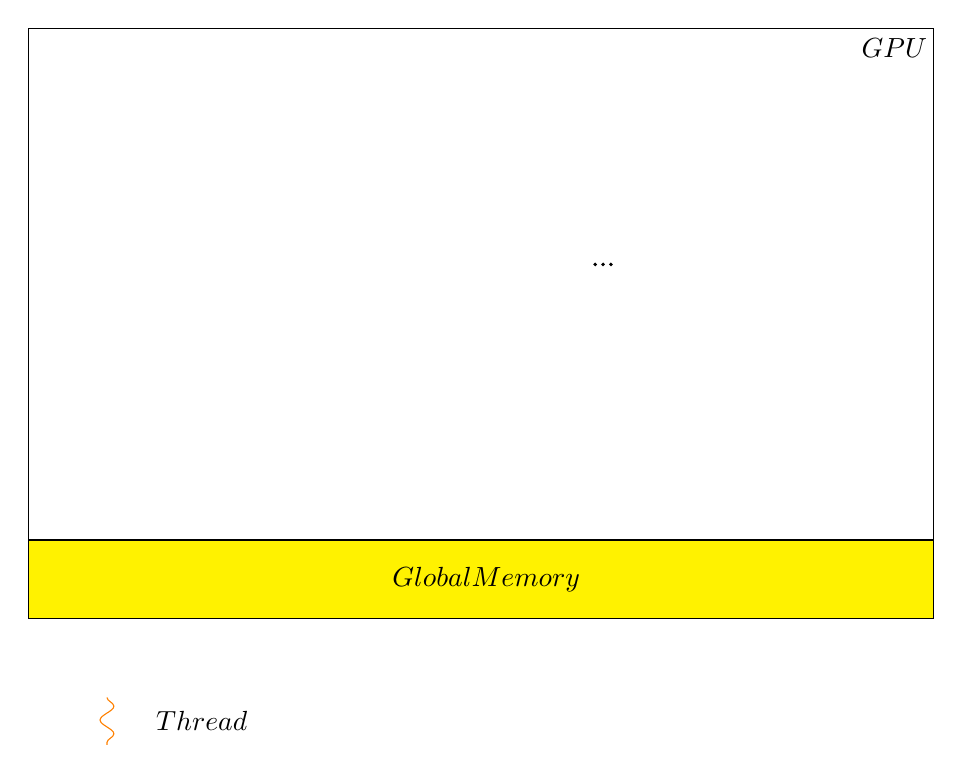
\begin{tikzpicture}
			
			\node[rectangle,
			draw = black,
			text = black,
			anchor = center,
			align=center,
			minimum width = 11.5cm, 
			minimum height = 7.5cm] (cpu1) at (3.75 cm, -0.75cm) {};
			\node[anchor=center] at (9 cm, 2.75 cm) {$GPU$};
			
			%\node[rectangle,
			%draw = black,
			%text = black,
			%anchor = center,
			%align=center,
			%minimum width = 11.5cm, 
			%minimum height = 1.5cm] (cpu1) at (3.75 cm, -6cm) {};
			%\node[anchor=center] at (9 cm, -5.5 cm) {$CPU$};
			
			
			\block{0}{0}{0}
			\block{3.2}{0}{1}
			\block{7.4}{0}{n}
			
			% Dots
			\node  at (5.2cm,0cm) [circle, fill, inner sep=0.5pt] {};
			\node  at (5.3cm,0cm) [circle, fill, inner sep=0.5pt] {};
			\node  at (5.4cm,0cm) [circle, fill, inner sep=0.5pt] {};
			
			
			\node[rectangle,
			draw = black,
			text = black,
			anchor = center,
			fill = yellow,
			align=center,
			minimum width = 11.5cm, 
			minimum height = 1cm] (cpu1) at (3.75 cm,-4cm) {};
			\node[anchor=west] at (2.5 cm, -4 cm) {$Global Memory$};
			
			\draw[orange, snake it] (-1 cm, -5.5cm) to
			(-1 cm, -6.1cm);
			
			\node[anchor=west] at (-0.5cm, -5.8) {$Thread$};
			
		\end{tikzpicture}
	\end{center}
\end{figure}

\subsubsection{Asynchronous Operations} \label{sec:async}

There are two types of engines that can be used to execute kernels in CUDA streams: copy engines and kernel engines. Copy engines are used to copy data between host and device memory, and between different types of memory on the device. Kernel engines are used to execute CUDA kernels. The number of individual engines depends on the actual hardware, lower end GPUs usually have a single kernel and a copy engine, more advanced architectures can have more than one copy or kernel engine.

A CUDA stream is a sequence of commands that are executed in order on a CUDA device. Streams can be used to improve the runtime of a CUDA program by overlapping the execution of different kernels. For example, a copy kernel can be executed in one stream while a compute kernel is executed in another stream. This overlap can lead to a significant performance improvement.


\subsubsection{Synchronization}

Whilst threads within a block can be synchronized, this is not the case for the blocks launched from a kernel. The only real synchronization technique, is to wait for a kernel, meaning all blocks associated with this kernel, to finish and execute a consecutive task using another kernel. 

Since the GPU is limited in its computing and also memory capabilities, the number of blocks which are run in parallel are limited, therefore CUDA cannot give us any guarantee, weather a set of blocks are run serially or in parallel. Some of the blocks might be run in parallel, meanwhile others are run serially. This very constraint, forces the programmer to rethink algorithms and think of ways, how individual subproblems can be run somewhat independently of each other. 

There exists however a way to communicate between blocks in a safe way. Atomic operations can be performed on global memory without any race conditions.

\subsection{Streams}

As described in section \ref{sec:async}, streams can be leveraged to improve the runtime a CUDA accelerated application. In the GPU accelerated ORB streams are used in a straight forward manner, each thread performs all its computations using its own unique stream. Since leveraging streams only improves the runtime in low numbers because the actual copy and kernel engines are not very numerous, this variant is very simple and effective. It was observed that using more streams on the individual threads does not improve the runtime, quiet contrary it can have a negative impact. 


\subsection{Memory Management}

Several strategies are used to improve the performance of memory allocation: 

\begin{enumerate}
	\item \textbf{Pinned Memory} As the GPU cannot access the default paged memory directly, when copying memory from the host to the device, the memory must first be copied to pinned memory. This means when pinned memory is used directly with $cudaMallocHost()$, data transfers can be around twice as fast. Thus pinned memory is used for all data, which needs to be either sent from the host to device or vice versa.
	\item \textbf{Reuse Memory} Memory allocation and freeing can be avoided altogether by reusing previously allocated memory whenever possible. Since there exists a fixed number of particles as well as an upper limit for the number of cells, memory can be allocated when calling the Initialize service and finalized with the Finalize service.
\end{enumerate}

\subsection{GPU Accelerated Count Left}

To solve the problem on the GPU essentially a general reduction can be taken as a basis and adapted to sum elements, which fulfill a certain condition. The condition is weather an element is than a given value, which in this case is the position of the cut plane. The code is based on the reduction as its explained in a Webinar from \textit{NVIDIA}. \cite{reduction}

\subsubsection{Schedule}

The entire schedule of the GPU accelerated ORB is depicted in figure \ref{fig:orbgpup}. In a first step the initialize service is called, where the necessary data is allocated on all devices and the particles are loaded. Furthermore the initial SPTDS is constructed, which essentially only consists of the root node, encompassing the entire domain and all the particles. Next the main loop of ORB is entered, which iterates until a SPTDS with the desired size is constructed. Within the loop the Count Service is called, computing the number of cells for each cell summed over all the threads in the system. To prepare the data for the GPU transfer a temporary array is made, using the make axis service, which is then sent to the GPU. 
At this stage the actual bisection methods starts on the master, where counting the number of particles left of a cut plane is done with the GPU Count Left service. Depending on the outcome, the cut position is improved respectively and the process is repeated until a nearly perfect cut is found for all the leaf cells of the current SPTDS. For each leaf cell cell two new child cells can be generated using the computed cut positions. Finally the SPTDS can be enriched with the new cell data and the particles array is partitioned accordingly using the Partition service. 
The tree building loop is then repeated or if the desired size of the SPTDS is reached, the loop is exited and the Finalize service is called to free the allocated memory.

\begin{figure}[H]
	\begin{center}
		\begin{tikzpicture}
			
			\timeline{6}{14}{3}
			
			
			\parallelloop{-2}{12.5}{8}{1.5}{loop till tree built};
			
			\parallelloop{-1}{9.5}{7}{5.5}{loop till cut found};
			
			\communication{Init}{0}{7}{13};
			
			\communication{Count}{0}{7}{12};
			
			\communication{Make Axis}{0}{7}{11};
			
			\communication{Copy Particles To GPU}{0}{7}{10};
			
			\communication{Count Left GPU}{0}{7}{9};
			
			\process{improve \\ cut}{0}{8};
			
			
			\process{generate\\ new \\ cells}{0}{5};
						
			\communication{Partition}{0}{7}{2};
			
			\communication{Finalize}{0}{7}{1};
			
			
		\end{tikzpicture}
	\end{center}
	\caption{Parallelized ORB GPU version}
	\label{fig:orbgpup}
\end{figure}

\subsubsection{Service}

The GPU version of the Count Left Service invokes the reduction kernel exactly once for every leaf cell of the current SPTDS. Meaning on level 0 of the tree there is only one kernel per processor being executed, when proceeding to further levels, the number of kernels is equivalent to $2^{depth}$ per processor. 
The number of blocks per cell can be determined by $N_{cell}$ divided by the number of threads per block and divided by the number of elements per thread, which is a strategy to increase the thread occupancy. 

All the relevant information can be passed along with the cell can be passed using pass by value  parameters, there is no need to copy any additional data from the CPU to the GPU in advance. The only relevant data is already in global memory, when the particles where copied from the host to the device. Hpwever the results, which are also stored in global memory, need to be copied back from the GPU to the GPU after the kernel has finished.

\subsubsection{Kernel Code}\label{sec:countleftcode}
The actual kernel code is depicted in listing \ref{cuda:reduction}. The input parameters of the reduction kernel (line 17-20) are: a pointer to the the particles stored in global memory, a pointer the an allocated array where the results are stored, the position of the cut plane and finally the total number of elements contained within the cell.

In a first step on lines 21-23 each thread ID \textit{tid} is associated with a pointer offset $i$ to the input data \textit{g\_idata}. Furthermore on line 25-26 the shared data is initialized and set to zero. Its size is equivalent to the block size, the total number of thread per block. Meaning there is room for a single float per thread in shared memory. On lines 28-30 the thread iterates over all elements which it is associated to and copies the results of a compare to shared memory. This allows us to work exclusively with shared memory instead of global memory, reducing the amount of costly memory accesses.

There exists an optimum in terms of number of operation performed by a single thread. In order to adapt the number of ops dynamically, the while loop ensures that each thread iterates over a certain number of elements as seen in lines 28-30. The input parameter \textit{n} defines the total number of particles. Therefore if the total number of blocks is reduced by a factor of $r$, the while loop will iterate over $r$ elements. Inside the while loop on line 27 the index $i$ is incremented by \textit{gridSize} in each iteration. The grid size is equivalent to the total number of threads associated with the kernel. Accessing the global memory in this pattern is coalesced but not necessarily aligned as the pointer of the input array probably does not start at a 32 index aligned address. \cite{gMem} \cite{reduction}

The rest of the kernel code performs the actual reduction, where in each step two elements from the shared memory are summed together. The exact pattern is chosen, because this way shared memory bank conflicts can be avoided, as each thread accesses only elements in shared memory which are stored in the same bank. \cite{sharedMem} Given a block size of 256, after line 39\footnote{lines 31-36 are not relevant as the block size is smaller than 512} exactly 256 sums are stored in shared memory. In a next step as seen on line 40 threads 0-127 in the block add the value stored at the same index in shared memory together with the values stored in a position which is offset by 128. This step reduces the total number of elements to be considered to 128, and the step can be repeated as seen on lines 45 to 48 until we reach 64 elements in shared memory which can be reduced by 32 threads. Meaning we only need to perform operations on a warp level which is done in the device kernel called \textit{warpReduce} as its invoked on line 51. 

The \textit{warpReduce} method takes the shared memory as an input and computes a reduction on warp level. Lines 5-6 perform a similar pattern as was seen before, but in this case we only need to synchronize among all threads in the warp using the \textit{\_syncwarp()} method. Finally we can perform the reduction on 32 elements by loading them to local memory and using the warp level primitive \textit{\_shfl\_down\_sync(m, v, o)}. The call gets the value of \textit{v} of thread with index offset by \textit{o} compared to the thread which calls the method. The mask \textit{m} specifies which threads should execute the function. Note that a non full mask this allows some form of divergence between threads in a warp without performance penalties. \cite{warps}

The reduction is optimized by using a template which takes as argument the total number of threads per block. Since the template is evaluated at compile time, all the if statements taking blockSize as a parameter in figure do not cause any performance loss. In fact, because  the reduction loops are unrolled (34-49) the the performance of the kernel is increased. \cite{reduction}

\begin{lstlisting}[language=c++, caption=Conditional Reduction in CUDA, label=cuda:reduction]
#define FULL_MASK 0xffffffff
template <unsigned int blockSize>
extern __device__ void warpReduce(
	volatile unsigned int *s_data, unsigned int tid) {
    if (blockSize >= 64) s_data[tid] += s_data[tid + 32];
	__syncwarp();
	if (tid < 32) {
		unsigned int val = s_data[tid];
		for (int offset = 16; offset > 0; offset /= 2)
			val += __shfl_down_sync(FULL_MASK, val, offset);
		s_data[tid] = val;
	}
}

template <unsigned int blockSize>
extern __global__ void reduce(
	float *g_idata,
	 unsigned int*g_odata, 
	 float cut, 
	 int n) {
	unsigned int tid = threadIdx.x;
	unsigned int i = blockIdx.x*(blockSize) + threadIdx.x;
	unsigned int gridSize = blockSize*gridDim.x;
	
	__shared__ int sdata[blockSize];
	sdata[tid] = 0;
	
	while (i < n) {
		sdata[tid] += (g_idata[i] <= cut);
		i += gridSize;
	}
	__syncthreads();
	
	if (blockSize >= 512) {
		if (tid < 256) {
			sdata[tid] += sdata[tid + 256];
		}
		__syncthreads();
	}
	if (blockSize >= 256) {
		if (tid < 128) {
			sdata[tid] += sdata[tid + 128];
		} __syncthreads();
	}
	if (blockSize >= 128) {
		if (tid < 64) {
			sdata[tid] += sdata[tid + 64];
		} __syncthreads();
	}
	if (tid < 32) {
		warpReduce<blockSize>(sdata, tid);
	}
	if (tid == 0) {
		g_odata[blockIdx.x] = sdata[0];
	}
}
\end{lstlisting}



Initializing the kernel once for each cell is a simple solution, however as the number of cells is increased, more calls to the kernel are made. Calls are not free of cost, as there is some overhead with each initialization of a kernel. Thus the performance degrades gradually as the tree is built, because on each level the number of cells for which the bisection method is executed doubles. At some point, the overhead even dominates over the actual computations by a lot. 


\subsection{Improved GPU Accelerated Count Left} \label{imprctl}

To solve the degrading performance problem some changes are made to the kernel and the overall schedule. The main idea is to prepare the necessary data for all cells in advance, effectively reducing the overall number of necessary kernel calls to $\lceil \log_2 d \rceil $ instead of $2 \times d$. In figure \ref{fig:degrading} the resulting number of kernel calls are compared for both versions. Each block is provided with information concerning the start and end index of the cells particles, the cut position as well as an index of the cell. 


\begin{figure}[H]
	\begin{center}
		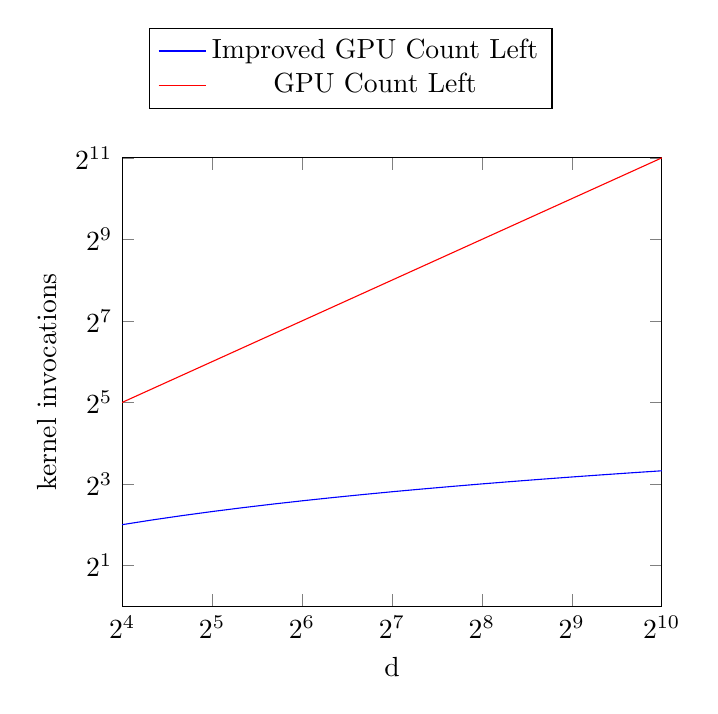
\begin{tikzpicture}
			\begin{axis}[
				xmode=log,
				ymode=log,
				log basis x={2},
				log basis y={2},
				xlabel={d},
				ylabel={kernel invocations},
				%x filter/.code=\pgfmathparse{#1 + 6.90775527898214},
				xmin = 16, xmax = 1024, ymin= 1, ymax=2048,
				legend style={at={(0.05,1.2)},anchor=west}]
				
				
				\addplot+[name path = A, domain = 16:4096, mark=none] {
					ln(\x) / ln(2) 
				};
				
				\addlegendentryexpanded{Improved GPU Count Left};
				
				\addplot+[name path = A, domain = 1:4096, mark=none] {
					2 * \x 
				};	
				
				\addlegendentryexpanded{GPU Count Left};
				
				
			\end{axis}
		\end{tikzpicture}
		\caption{Kernel calls with GPU count left versions}
		\label{fig:degrading}
	\end{center}
\end{figure}

The improved Count Left service works as follows on a simple example: Given $cell_2$ with a volume that encompasses particles in the range 0 - 10240 and $cell_3$ encompasses particles in the range 10240 - 20480.  A block size of 256 threads is given and the number of elements per thread is set to 16, thus each block processes $256 * 16 = 4096$ elements. In this case two blocks are allocated to each cell, where the first block processes elements 0 - 4096 and the second one 4096 - 10240. By assigning more work to the second block, the threads will perform more work as others, however this is more favorable than threads which perform less work. Furthermore blocks where not even all the threads are occupied can be avoided that way. Consequently the third and fourth block respectively process particles 10240 to 14446 and 14446 to 20480. Since the number of required blocks for cell is known as well as the exact range of particles for which the reduction has to be computed, all this information can be copied to the GPU in advance and a kernel with the total block sum can be launched. 
Each kernel stores its information in an output array where the assignment between the output and the actual cell is known. The service therefore needs to iterate over all the output which have been computed by the blocks associated with a kernel and output them at a single cell specific location in the output $ou$ array of the service.

\subsubsection{Schedule}

Only a single change is made to the schedule: A service called GPU Copy Cell Service is introduced, which does as the name says, copies the cell information from the CPU to the GPU. Since only the cut positions change while ORB is iterating to find and improve a cut and the rest of the cell information stays static, this service can be called outside of the loop. The Improved GPU Count Left Service copies the cut data each time it is invoked. Other than that, the schedule remains equal. 

\begin{figure}[H]
	\begin{center}
		\begin{tikzpicture}
			
			\timeline{6}{15}{3}
			
			
			\parallelloop{-2}{13.5}{8}{1.5}{loop till tree built};
			
			\parallelloop{-1}{9.5}{7}{5.5}{loop till cut found};
			
			\communication{Init}{0}{7}{14};
			
			\communication{Count}{0}{7}{13};
			
			\communication{Make Axis}{0}{7}{12};
			
			\communication{Copy Particles To GPU}{0}{7}{11};
			
			\communication{Copy Cells To GPU}{0}{7}{10};
			
			\communication{Improved Count Left GPU}{0}{7}{9};
			
			\process{improve \\ cut}{0}{8};
			
			
			\communication{Partition}{0}{7}{5};
			
			\communication{Finalize}{0}{7}{1};
			
			\process{generate\\ new \\ cells}{0}{4};
			
		\end{tikzpicture}
	\end{center}
	\caption{Parallelized ORB GPU version 2}
	\label{fig:orbgpup2}
\end{figure}


\subsubsection{Kernel Code}

The kernel code as seen in listing \ref{ctlocuda} largely remains the same. New data pointers are passed along as a parameter where $g_begin$ and $g_end$ mark the begin and end of the important particle array slice, furthermore $g_cuts$ is an array of cell cuts for each block. The data is prepared in such a way, that each block only needs to operate over the particles contained within a single cell. $blockIdx.x$ provides the index to read out the cell information from the input arrays (lines 20 - 22). Everything else, including the subroutine $warpReduce$ remains equal. 

\begin{figure}[H]
	\begin{lstlisting}[language=c++, caption=Kernel Optimized GPU Count Left, label = ctlocuda]
template <unsigned int blockSize>
extern __global__ void reduce(
float * g_idata,
unsigned int * g_begins,
unsigned int * g_ends,
float * g_cuts,
unsigned int * g_odata) {
	__shared__ unsigned int s_data[blockSize];
	
	unsigned int tid = threadIdx.x;
	const unsigned int begin = g_begins[blockIdx.x];
	const unsigned int end = g_ends[blockIdx.x];
	const float cut = g_cuts[blockIdx.x];
	
	unsigned int i = begin + tid;
	s_data[tid] = 0;
	
	// unaligned coalesced g memory access
	while (i < end) {
		s_data[tid] += (g_idata[i] <= cut);
		i += blockSize;
	}
	__syncthreads();
	
	if (blockSize >= 512) {
		if (tid < 256) {
			s_data[tid] += s_data[tid + 256];
		}
		__syncthreads();
	}
	if (blockSize >= 256) {
		if (tid < 128) {
			s_data[tid] += s_data[tid + 128];
		} __syncthreads();
	}
	if (blockSize >= 128) {
		if (tid < 64) {
			s_data[tid] += s_data[tid + 64];
		} __syncthreads();
	}
	if (tid < 32) {
		warpReduce<blockSize>(s_data, tid);
	}
	if (tid == 0) {
		g_odata[blockIdx.x] = s_data[0];
	}
}
	\end{lstlisting}
	\caption{Reduction in CUDA}
	\label{cuda:reduction2}
\end{figure}


\subsection{Improved GPU Accelerated Count Left with Warp Level Primitives} \label{imprctlwrp}

The above described kernel code can also be rewritten where warp level primitives are leveraged to the full extent. Lines 1-14 are identical as in the previous kernel as proposed in listing \ref{ctlocuda}.
On lines 16 and 17 we fetch the lane $id$ and the $warpId$. The $lane$ defines the index of a thread inside each warp. The operation $tid \& (32 - 1)$ is equivalent to $tid \% 32$ but significantly faster \cite{bestp}.
When incrementally assigning an index to each warp the index can be fetched by dividing the $tid$ by the number of threads in a warp, which is then implicitly floored when converted into an integer. The operation $tid >> 5$ is equivalent to $tid / 32$ \cite{bestp}.

Instead of iterating over elements and storing them in global memory, the data is stored in local memory as seen on lines 19 to 24. Furthermore, at this stage there is no need to sync all threads within the block but only the threads within a warp, therefore the command \textit{\_syncthreads()} can be replaced with \textit{\_syncwarp()}.
On lines 26 - 27 a warp level reduction is performed, which is equivalent to the one we have explained with the previous kernel. Now each tread with a $lane$ equivalent to 0 has stored the sum of 31 next consecutive threads. In the case of 256 threads this means that there are 8 elements left to be summed up, however this step cannot be performed on a warp level as all the elements are stored in threads from distinct warps or unique $warpId$. Therefore the $val$ stored in local memory is stored to shared memory at the $warpId$ index and a \textit{\_syncthreads()} call is made (line 29-32). In this case it necessary to synchronize all threads, as the storing of elements happens across warps.
Finally all threads within the very first warp, meaning the ones with a $warpId$ of 0, reload the data from shared to local memory and a final warp level reduction can be performed (lines 34-41). A single element on thread 0 stores now the entire sum across all input data elements and it can be written to global memory and later fetched from the CPU.

\begin{figure}[H]
	\begin{lstlisting}[language=c++, caption=Kernel Optimized GPU Count Left,
		label = ctlocudawrp]
template <unsigned int blockSize>
extern __global__ void reduce3(
float * g_idata,
unsigned int * g_begins,
unsigned int * g_ends,
float * g_cuts,
unsigned int * g_odata) {
	__shared__ unsigned int s_data[32];
	unsigned int tid = threadIdx.x;
	const unsigned int begin = g_begins[blockIdx.x];
	const unsigned int end = g_ends[blockIdx.x];
	const float cut = g_cuts[blockIdx.x];
	unsigned int i = begin + tid;
	s_data[tid] = 0;
	
	const unsigned int lane = tid & (32 - 1);
	const unsigned int warpId = tid >> 5;
	
	unsigned int val = 0;
	while (i < end) {
		val += (g_idata[i] <= cut);
		i += blockSize;
	}
	__syncwarp();
	
	for (int offset = 16; offset > 0; offset >>= 1)
		val += __shfl_down_sync(FULL_MASK, val, offset);
	
	if (lane == 0) {
		s_data[warpId] = val;
	}
	__syncthreads();
	
	if (warpId == 0) {
		val = 0;
		if (tid < 32 && tid * 32 < blockSize) {
			val += s_data[tid];
		}
		
		for (int offset = 16; offset > 0; offset >>= 1)
			val += __shfl_down_sync(FULL_MASK, val, offset);
		
		if (tid == 0) {
			g_odata[blockIdx.x] = val;
		}
	}
}
	\end{lstlisting}
	\caption{Reduction in CUDA}
	\label{cuda:reduction3}
\end{figure}



\subsection{GPU Accelerated Partitioning}

A GPU accelerated Count Left service is implemented successfully. Since the particles are still partitioned on the CPU, the data needs to be copied to GPU each time the SPTDS is expanded. As the Make Axis service is used to compress the axes into a single array, only $N$ elements need to be copied, but this needs to be repeated $\lceil \log_2 d \rceil$ times. 
If the particles are partitioned on the GPU, it needs to be copied only once, but in this case all three coordinates have to be copied, thus $
N \times 3$. Nevertheless this corresponds a fraction of the total data transfer: $\frac{3}{\lceil \log_2 d \rceil \times}$. In figure \ref{fig:transfer} its observable that a GPU partition becomes feasible, at least in terms of data transfer, after $d$ exceeds 16. 

\begin{figure}[H]
	\begin{center}
		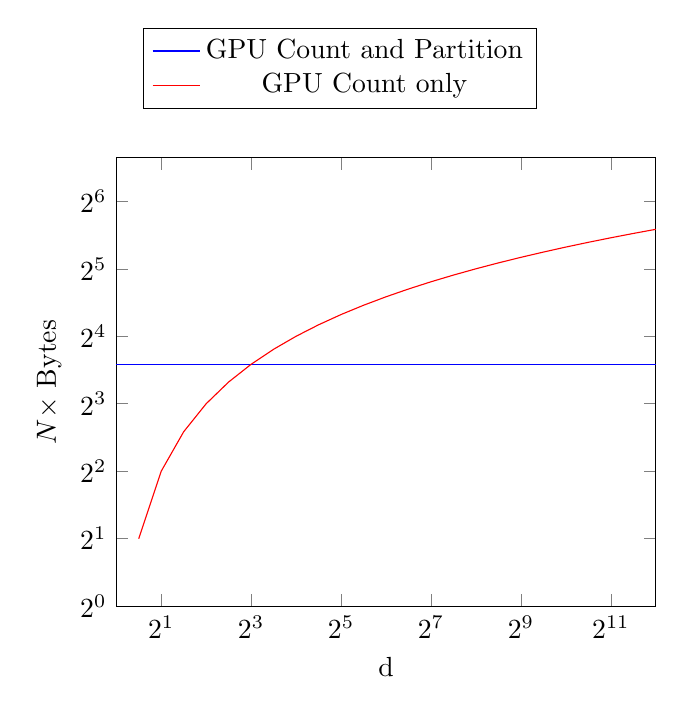
\begin{tikzpicture}
			\begin{axis}[
				xmode=log,
				ymode=log,
				log basis x={2},
				log basis y={2},
				xlabel={d},
				ylabel={$N \times$ Bytes},
				%x filter/.code=\pgfmathparse{#1 + 6.90775527898214},
				xmin = 1, xmax = 4096, ymin= 1, ymax=100,
				legend style={at={(0.05,1.2)},anchor=west}]
				

				\addplot+[name path = A, domain = 1:4096, mark=none] {
					3 * 4
				};
			
				\addlegendentryexpanded{GPU Count and Partition};
			
				\addplot+[name path = A, domain = 1:4096, mark=none] {
					ln(\x) / ln(2) * 4
				};	
				
				\addlegendentryexpanded{GPU Count only};

				
			\end{axis}
		\end{tikzpicture}
		\caption{Data transferred with and without GPU partitioning}
		\label{fig:transfer}
	\end{center}
\end{figure}


A GPU partitioning algorithm was first proposed by Cederman \cite{GPUQ} and later refined by Manca \cite{CUDAQ} where atomic operations are leveraged to improve the runtime of the algorithm. This version is built around the concepts introduced by Manca. 

Early results have shown partitioning the data on the GPU is not really faster than the CPU version where the CPU version is not even implemented in a optimal manner and finally the number of particles which can be stored on the GPU memory is reduced by $\frac{5}{3}$. This is caused by required additional temporary arrays for memory swaps on the GPU. Furthermore there was not enough time to fully optimize and track down all issues with the code, therefore not full kernel code is provided, instead the underlying concepts are introduced for subsequent work. 

\subsubsection{Schedule}

In the adapted schedule (figure \ref{fig:orbgpu3}) the Copy Particles To GPU service can be moved out of the main loop. Other than that the schedule remains the same. 

\begin{figure}[H]
	\begin{center}
		\begin{tikzpicture}
			
			\timeline{6}{14}{3}
			
			
			\parallelloop{-2}{11.5}{8}{1.5}{loop till tree built};
			
			\parallelloop{-1}{9.5}{7}{5.5}{loop till cut found};
			
			\communication{Init}{0}{7}{13};
			
			\communication{Copy Particles To GPU}{0}{7}{12};
			
			\communication{Count}{0}{7}{11};
		
			
			\communication{Copy Cells To GPU}{0}{7}{10};
			
			\communication{Count Left GPU}{0}{7}{9};
			
			\process{improve \\ cut}{0}{8};
			
			
			\communication{Partition}{0}{7}{5};
			
			\communication{Finalize}{0}{7}{1};
			
			\process{generate\\ new \\ cells}{0}{4};
			
		\end{tikzpicture}
	\end{center}
	\caption{Parallelized ORB with GPU counting and GPU partitioning}
	\label{fig:orbgpu3}
\end{figure}


\subsubsection{Partitioning a Single Cell}

In a first step a block wise partition is performed, meaning there is no synchronization between blocks at this stage. Each thread loads the particle coordinate of the matching axis into the shared memory register $S$. Then two copies of the data stored in the shared memory are made where the first copy $A$ compares each value with the cut and stores 0 if the value is smaller and 1 otherwise. Consequently the second copy $B$ stores the inverted result. 
Now a parallel prefix sum\footnote{Commonly refered to as a scan} is computed on both copies, where an algorithm as described in GPU Gems \cite{SCAN} can be used. In $B$ each element is then incremented by the an offset equal to the total number of elements smaller than the cut. 
In theory the block wise partition could already be applied by storing each element with index $i$ larger than the cut at $A_i$ and larger elements at $B_i$. 
However the goal is to partition all elements across multiple blocks. To do so a global variable called $leq$ and $g$ is introduced, where the total number of elements smaller equal and bigger than the cut are stored. Each time a block has computed both scans, the number of elements designated to the block smaller and larger than the cut are known. Thus a single thread of each block performs an atomic add on $leq$ and $g$ accordingly. $AtomicAdd()$ returns the old value of the variable. The return value can be caught and stored two designated shared memory register $s_leq$ and $s_g$. 
At this stage every thread in a block agrees on a value for $s_leq$ and $s_g$ the values can be treated as starting indices to store the block wise partitioned results in the output array. In this case however an element $i$, which is larger than the cut is stored location $A_i + s_leq$ and if larger at $B_i = s_g$. 

In this case the input array are coordinate values of particles and the output array is a temporary array of size $N$. The in an output array cannot be the same as the partition cannot be performed in place. Doing so would result in elements that are overwritten before they are read by the thread assigned to it. This cannot be avoided with the proposed technique as the relationship between the range of input data treated by a kernel and the output is not deterministic. Its dictated by the order, by which the kernel reach the $atomicAdd()$ statement. 

As of now only a single axis is partitioned, but the same needs to be done for the other two axes. One approach is to partition all the other arrays in the same kernel, as the permutations can simply be reapplied. However in this case three  additional temporary arrays are needed, one for each axis. Further Reducing the number of particles which can be stored on the GPU by $\frac{1}{2}$. A more memory efficent, but slightly slower variant is to allocate another array on the GPU where the actual permutation indices are stored when the partition kernel is executed. Therefore together with the temporary array $N$ is only reduced by $\frac{3}{5}$. After the partition kernel has finished, the coordinates can be copied back from the temporary array to the original location in a device to device copy. Then the second axis is partitioned using the precomputed permutations and the results are again copied back to the proper location. Finally after the step is repeated for the last axis, the partition is finished.

\subsubsection{Partitioning Multiple Cells}

The same method as introduced in section \ref{imprctl} is applied to ensure only a single kernel has to be launched for all cells. 
Each block is assigned a cell, where all relevant information about the cell is stored in different arrays in global memory. Each block then read the designated data by acessing the arrays at index $blockIdx.x$. The variables $leq$ and $g$ are replaced by arrays of the same length as there are cells to be partitioned\footnote{which is not equivalent to the total number of blocks}. This ensures all the blocks assigned to a single cell perform the atomic operations on the same variable. For a block to know which element in the $leq$ and $g$ arrays it needs to access, a sequential cell index array is passed, where all blocks working on the same cell receive the same cell index. 


\newpage
\section{Performance Analysis of ORB}\label{sec:empan}

All measurements where performed on Piz Daint where the performance of system can be read from table \ref{fig:datapoints}.

\begin{figure}[H]
	\begin{center}
		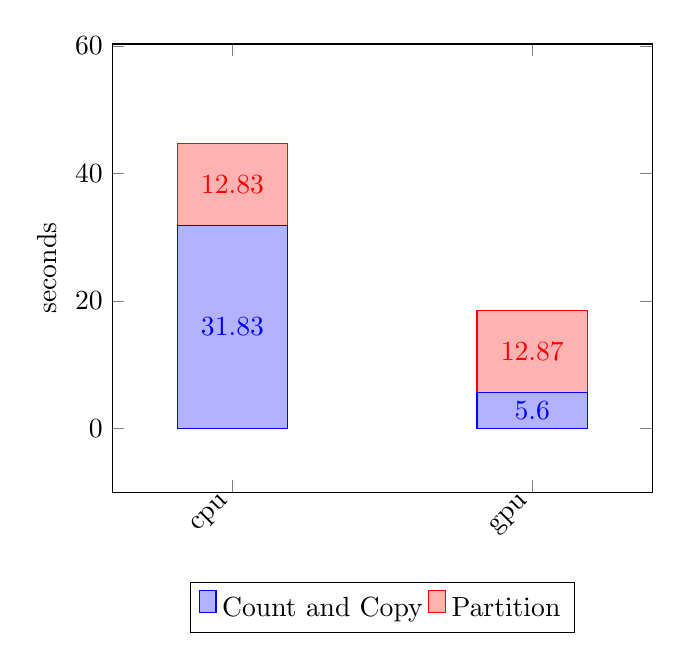
\begin{tikzpicture}
			
			\begin{axis}
				[
				 enlargelimits=0.4,
				ybar stacked,
				bar width=40pt,
				nodes near coords,
				legend style={at={(0.5,-0.20)},
					anchor=north,legend columns=-1},
				ylabel={seconds},
				symbolic x coords={cpu, gpu},
				xtick=data,
				x tick label style={rotate=45,anchor=east}]
				ymin=0,
				ymax=50
				]
				\addplot+[ybar] plot coordinates {(cpu, 31.83) (gpu, 5.60)};
				\addplot+[ybar] plot coordinates {(cpu, 12.83) (gpu, 12.87)};

			\legend{\strut Count and Copy, \strut Partition}
			\end{axis}
			
			
		\end{tikzpicture}
	\end{center}
	
	\caption{Execution times of different strategies}
	\label{fig:analy2}
\end{figure}

In figure \ref{fig:analy2} the final measurements are plotted. The total runtime of the ORB is around 43 seconds when performed only on the CPU, for the GPU accelerated version it comes down to 18 seconds. However a large part of the execution time can be attributed to the Partitioning, where its overhead remains equal for both versions. Even the CPU Partitioning can be improved a lot and the GPU version might increase the performance even further. 
If the time lost during the partitioning is subtracted, the GPU version is about $5.6$ times faster, which is slightly worse than the expected speedup of $6.2$. The difference can be explained by additional overheads, especially as the GPU kernel has to touch the elements more than once due to the way it was implemented. 

When looking at the absolute number there is a stark difference: $56.47s$ predicted for the CPU version were $31.83$ was the actual timing. Similarly the GPU was expected to execute ORB\footnote{Excluding the time required for the partition} in $8.99s$, however it only took $5.6s$. The theoretical model considers an upper bound for the total number of iterations which the bisection method takes to converge. In reality this number is closer to 20 than to $p$ which is 32 in the measured data. When considering this, the measurements are also in an absolute term relatively close to the theoretical model. $56.47s \times \frac{20}{32} = 37s$ against the actual $31.83s$ and $8.99s \times \frac{20}{32} =5.99s$ compared to $5.6s$.
\subsection{Scaling}

To make sure the GPU version scales well the runtime were evaluated for different number of particles. 


\begin{filecontents*}{results0.csv}
	p, d, t, t2
	1048576, 10, 0.04
	4194304, 10, 0.14
	16777216, 10, 0.61
	67108864, 10, 2.57
	268435456, 10, 11.15
	1073741824, 10, 47.58, 
\end{filecontents*}

\begin{filecontents*}{results1.csv}
	p, d, t, t2
	1048576 , 10, 0.04
	4194304, 10, 0.10
	16777216 , 10, 0.33
	67108864 , 10, 1.24
	268435456 , 10, 4.98
	1073741824, 10, 20.31
\end{filecontents*}

\begin{figure}[H]
	\begin{center}
		\begin{tikzpicture}
			
			\begin{axis}
				[
				xlabel={number of particles},
				ylabel={seconds},
				nodes near coords,
				xmin=1048576,
				xmax=1073741824,
				ymin=0,
				ymax=64,
				xmode=log,
				ymode=log,
				log basis x={2},
				log basis y={2},
				legend style={at={(1.05,0.6)},anchor=west}]
				]
				\addplot+[
				point meta=explicit symbolic
				] table [
				x=p, 
				y=t, 
				col sep=comma] 
				{results0.csv};
				\addlegendentryexpanded{CPU Only};
				\addplot+[
				point meta=explicit symbolic
				] table [
				x=p, 
				y=t, 
				col sep=comma] 
				{results1.csv};
				\addlegendentryexpanded{GPU Count Left};
			\end{axis}
			
			
		\end{tikzpicture}
	\end{center}
	
	\caption{Execution times of different strategies}
	\label{fig:analy}
\end{figure}

\newpage
\section{Conclusion}

In the thesis I explored how the ORB method works in detail, I established solid knowledge about different ways to estimate the performance of computer. Using the foundation I have built estimates for a CPU and two GPU accelerated versions of ORB. Furthermore I have bolstered my experience in C++ programming and learned the most important theoretical foundations about CUDA. Using all the gained knowledge I have looked at numbers CUDA source codes and blog articles to come up with an efficient reduction kernel which works well with segmented problems where each segment requires a different reduction strategy. I have implemented a GPU partitioning where early results and time constraints lead to an unfinished implementation, nevertheless the concept should work and could potentially lead to further performance improvement in ORB. 
When isolating the time it takes to compute a cut, without considering the time used for partitioning, the GPU accelerated version I have implemented runs about 5.6 times faster than a fully optimized and parallelized CPU version. 
 


% Use for reduction explanation https://texample.net/tikz/examples/database-decimation-process/
%\bibliographystyle{unsrt}
\newpage
\bibliography{reference}


\listoffigures
\listoftables

\end{document}
